\chapter{曲线}

\section{引言}

曲线和曲面的微分几何有两个方面.一个方面，可以称为经典微分几何，始于微积分的开端.粗略地说，经典微分几何是研究曲线和曲面的局部性质.我们所说的局部性质是指那些仅取决于曲线或曲面在某点邻域行为的性质.在研究这些性质方面被证明是足够的方法是微分学的计算方法.因此，微分几何中考虑的曲线和曲面将由可以进行一定次数微分的函数定义.

另一方面是所谓的整体微分几何.这里研究的是局部性质对整个曲线或曲面行为的影响.我们将在本书后面回到微分几何的这一方面.

也许经典微分几何中最有趣和最具代表性的部分是曲面研究.然而，在研究曲面时，一些曲线的局部性质自然会出现.因此，我们将使用本章对曲线进行简要处理.

本章的组织方式是，主要对曲面感兴趣的读者可以只阅读第1-2节至第1-5节.第1-2节至第1-4节包含基本介绍性材料(参数化曲线、弧长、向量积)，这些内容可能已从其他课程中了解，在此包含是为了完整性.第1-5节是本章的核心，包含研究曲面所需的曲线材料.对于希望在曲线主题上更进一步的读者，我们包含了第1-6节和第1-7节.

\section{参数化曲线}

我们将 $\mathbb{R}^3$ 记为实数三元组 $(x,y,z)$ 的集合.我们的目标是刻画 $\mathbb{R}^3$ 的某些子集(称为曲线)，这些子集在某种意义上是一维的，并且可以应用微分学的计算方法.定义这类子集的自然方式是通过可微函数.我们称实变量实函数是可微的(或光滑的)，如果它在所有点都具有所有阶的导数(这些导数自动是连续的).曲线的第一个定义，虽然不完全令人满意，但足以满足本章的目的，如下所示.

\begin{definition}{参数化可微曲线}
    参数化可微曲线是实数线 $\mathbb{R}$ 的开区间 $I = (a,b)$ 到 $\mathbb{R}^3$ 的可微映射 $\alpha  : I \rightarrow  \mathbb{R}^3$ .
\end{definition}


此定义中的可微意味着 $\alpha$ 是一个映射，将每个 $t \in  I$ 映射到点 $\alpha(t)  = (x(t) ,y(t) ,z(t))  \in  \mathbb{R}^3$ ，使得函数 $x(t) ,y(t) ,z(t)$ 是可微的.变量 $t$ 称为曲线的参数.区间一词采用广义的含义，因此我们不排除 $a =  - \infty ,b =  + \infty$ 的情况.

如果我们用 $x'(t)$ 表示 $x$ 在点 $t$ 处的第一导数，并对函数 $y$ 和 $z$ 使用类似的记法，则向量 $(x'(t) ,y'(t) ,z'(t))  = \alpha'(t)  \in  \mathbb{R}^3$ 称为曲线 $\alpha$ 在 $t$ 处的切向量(或速度向量).图像集 $\alpha(I)  \subset  \mathbb{R}^3$ 称为 $\alpha$ 的轨迹.正如下面的示例 5 所说明的，应该仔细区分参数化曲线(一个映射)与其轨迹( $\mathbb{R}^3$ 的一个子集).

关于术语的警告.许多人使用“无限可微”一词来表示具有所有阶导数的函数，而将“可微”一词保留为仅要求存在第一导数.我们不遵循这种用法.

\begin{instance}
    由以下公式给出的参数化可微曲线

    \[\alpha(t)  = (a\cos t,a\sin t,bt) ,\;t \in  \mathbb{R},\]

    在 $\mathbb{R}^3$ 中的轨迹是一个螺旋线，其螺距为 $2\pi b$ ，位于圆柱体 $x^2 + y^2 = a^2$ 上.这里的参数 $t$ 表示 $x$ 轴与连接原点 0 与点 $\alpha(t)$ 在 $xy$ 平面上的投影的直线之间的夹角(见图 1-1).
\end{instance}



\begin{figure}[h]
    \centering
    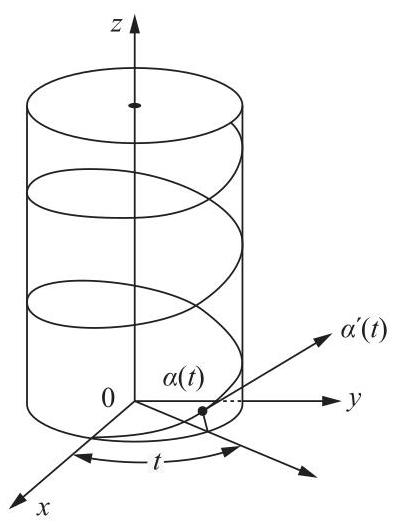
\includegraphics[max width=0.3\textwidth]{images/1.1.jpg}
    \captionof{figure}{螺旋线}
\end{figure}
\hspace*{3em} 

\begin{figure}[h]
    \centering
    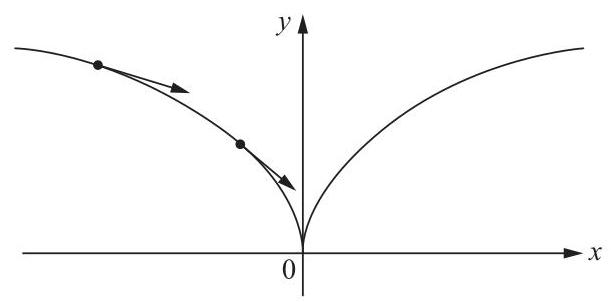
\includegraphics[max width=0.5\textwidth]{images/1.2.jpg}
    \captionof{figure}{尖点}
\end{figure}
\hspace*{3em} 



\begin{instance}
    由 \(\alpha \left( t\right)  = \left( {{t}^{3},{t}^{2}}\right) ,t \in  R\) 给出的映射 \(\alpha  : R \rightarrow  {R}^{2}\) 是一个参数化可微曲线，其轨迹如图 1-2 所示.请注意， \({\alpha }^{\prime }\left( 0\right)  = \left( {0,0}\right)\) ；也就是说，对于 \(t = 0\) ，速度向量为零.
\end{instance}
\begin{instance}
    由 \(\alpha \left( t\right)  = \left( {{t}^{3} - {4t},{t}^{2} - 4}\right)\) 和 \(t \in  R\) 给出的映射 \(\alpha  : R \rightarrow  {R}^{2}\) 是一个参数化可微曲线(见图 1-3).请注意， \(\alpha \left( 2\right)  = \alpha \left( {-2}\right)  = \left( {0,0}\right)\) ；也就是说，映射 \(\alpha\) 不是一对一的.
    \begin{center}
    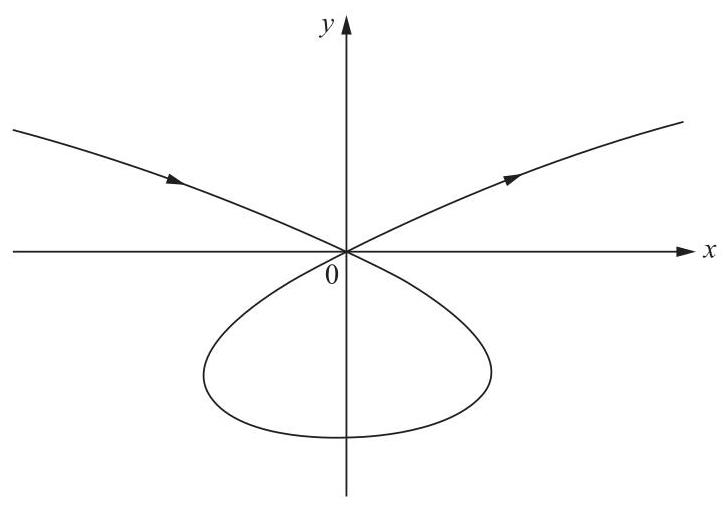
\includegraphics[max width=0.6\textwidth]{images/1.3.jpg}
    \captionof{figure}{图 1-3}
    \end{center}
\end{instance}




\begin{instance}
    由 $\alpha(t)  = (t,|t|),t \in  \mathbb{R}$ 给出的映射 $\alpha  : \mathbb{R} \rightarrow  \mathbb{R}^2$ 不是参数化可微曲线，因为 $|t|$ 在 $t = 0$ 处不可微(图 1-4).
    \begin{center}
    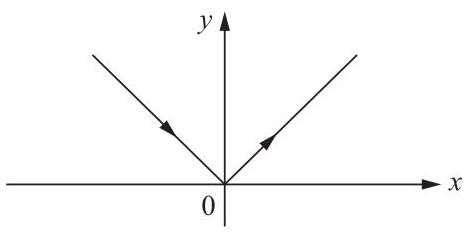
\includegraphics[max width=0.4\textwidth]{images/1.4.jpg}
    \captionof{figure}{图 1-4}
    \end{center}
\end{instance}

\begin{instance}
    两个不同的参数化曲线
    \begin{align*}
        \alpha(t)  = (\cos t &,\sin t) \\
        \beta(t)  = (\cos 2t &,\sin 2t)
    \end{align*}
    其中 $t \in  (0 - \varepsilon ,2\pi  + \varepsilon ),\varepsilon  > 0$ ，具有相同的轨迹，即圆 $x^2 + y^2 = 1$ .注意第二条曲线的速度向量是第一条曲线的两倍(图 1-5).
    \begin{center}
    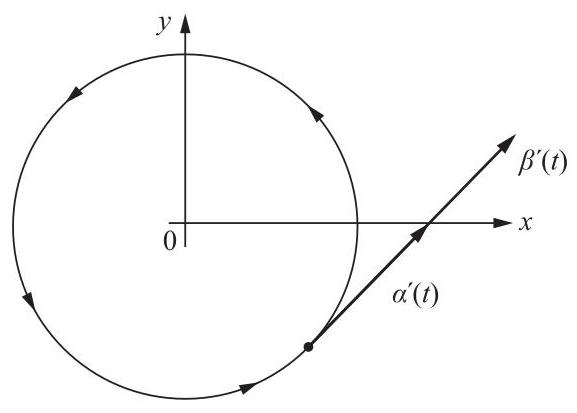
\includegraphics[max width=0.5\textwidth]{images/1.5.jpg}
    \captionof{figure}{图 1-5}
    \end{center}
\end{instance}



现在我们简要回顾一下向量在 $\mathbb{R}^3$ 中的内积(或点积)的一些性质.设 $u = (u_1,u_2,u_3)  \in  \mathbb{R}^3$ 并定义其范数(或长度)为

\[
|u|  = \sqrt{u_1^2 + u_2^2 + u_3^2}.
\]

几何上， $|u|$ 是点 $(u_1,u_2,u_3)$ 到原点 $O = (0,0,0)$ 的距离.现在，设 $u = (u_1,u_2,u_3),v = (v_1,v_2,v_3)\in\mathbb{R}^3$ ，设 $\theta ,0 \leq  \theta  \leq  \pi$ 是由线段 $Ou$ 和 $Ov$ 形成的夹角.内积 $u \cdot  v$ 定义为(图 1-6)

\[
u \cdot  v = |u| |v| \cos \theta .
\]

以下性质成立:
\begin{enumerate}
    \item 假设 $u$ 和 $v$ 是非零向量.则 $u \cdot  v = 0$ 当且仅当 $u$ 与 $v$ 正交.
    \item $u \cdot  v = v \cdot  u$ .
    \item $\lambda(u \cdot  v)  = (\lambda u) \cdot  v = u \cdot  (\lambda v)$ .
    \item $u \cdot  (v + w)  = u \cdot  v + u \cdot  w$ .
\end{enumerate}
可以通过以下方式获得内积的有用表达式.设 $e_1 = (1,0,0) ,e_2 = (0,1,0)$ ，和 $e_3 = (0,0,1)$ .很容易检查


\begin{center}
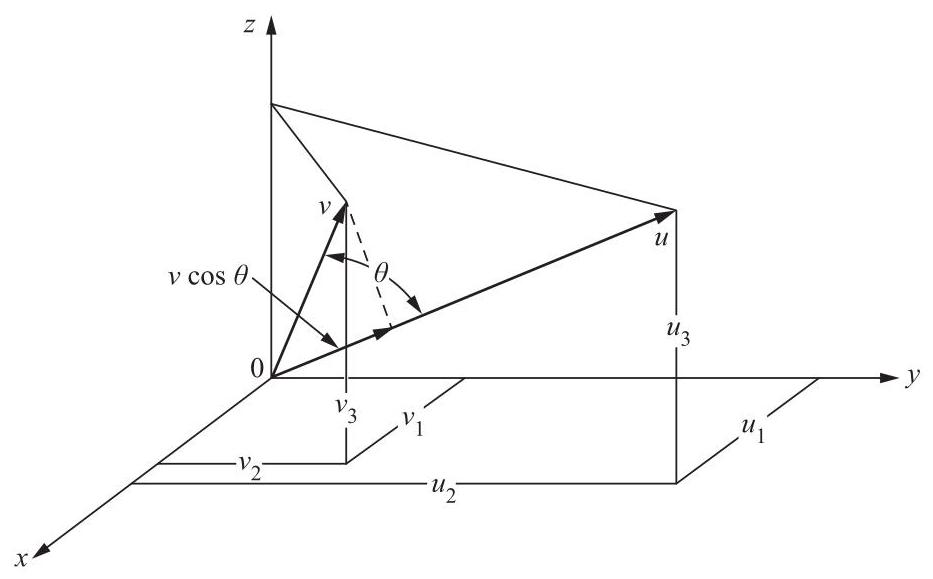
\includegraphics[max width=0.8\textwidth]{images/1.6.jpg}
\captionof{figure}{图 1-6}
\end{center}

当 $e_i \cdot  e_j = 1$ 如果 $i = j$ 并且 $e_i \cdot  e_j = 0$ 如果 $i \neq  j$ ，其中 $i,j = 1,2,3$ .因此，通过写

\[
u = u_1e_1 + u_2e_2 + u_3e_3,\;v = v_1e_1 + v_2e_2 + v_3e_3,
\]

并使用性质 2 到 4，我们得到

\[
u \cdot  v = u_1v_1 + u_2v_2 + u_3v_3.
\]

从上述表达式可知，如果 $u(t)$ 和 $v(t) ,t \in  I$ 是可微曲线，则 $u(t)  \cdot  v(t)$ 是可微函数，并且

\[
\frac{d}{dt}(u(t)  \cdot  v(t))  = u'(t)  \cdot  v(t)  + u(t)  \cdot  v'(t) .
\]

\exerciseline
\begin{enumerate}
    \item 找到一条参数化曲线 $\alpha(t)$ ，其轨迹是圆 $x^2 + y^2 = 1$ ，使得 $\alpha(t)$ 沿圆顺时针方向运动，且 $\alpha(0)  = (0,1)$ .
    \item 设 $\alpha(t)$ 是一条不通过原点的参数化曲线.如果 $\alpha(t_0)$ 是 $\alpha$ 的轨迹上离原点最近的点，并且 $\alpha'(t_0)  \neq  0$ ，则位置向量 $\alpha(t_0)$ 与 $\alpha'(t_0)$ 正交.
    \item 一个参数化曲线 $\alpha(t)$ 具有其二阶导数 $\alpha''(t)$ 恒等于零的性质.关于 $\alpha$ 可以说什么？
    \item 令 $\alpha  : I \rightarrow  \mathbb{R}^3$ 为一个参数化曲线，令 $v \in  \mathbb{R}^3$ 为一个固定向量.假设对于所有 $t \in  I$ ， $\alpha'(t)$ 都与 $v$ 正交，并且 $\alpha(0)$ 也与 $v$ 正交.证明对于所有 $t \in  I$ ， $\alpha(t)$ 都与 $v$ 正交.
    \item 令 $\alpha  : I \rightarrow  \mathbb{R}^3$ 为一个参数化曲线，对于所有 $t \in  I$ 都有 $\alpha'(t)  \neq  0$ .证明当且仅当对于所有 $t \in  I$ ， $\alpha(t)$ 与 $\alpha'(t)$ 正交时， $|\alpha(t)|$ 是一个非零常数.
\end{enumerate}

\section{正则曲线；弧长}

令 $\alpha  : I \rightarrow  \mathbb{R}^3$ 为一个参数化可微曲线.对于每个 $t \in  I$ (其中 $\alpha'(t)  \neq  0$ )，存在一条明确定义的直线，该直线包含点 $\alpha(t)$ 和向量 $\alpha'(t)$ .这条直线称为 $\alpha$ 在 $t$ 处的切线.对于研究曲线的微分几何来说，在每一点都存在这样的切线是至关重要的.因此，我们将 $\alpha'(t)  = 0$ 的任何点 $t$ 称为 $\alpha$ 的奇异点，并将注意力限制在没有奇异点的曲线上.注意，在 1-2 节的示例 2 中，点 $t = 0$ 是一个奇异点.

定义.一个参数化可微曲线 $\alpha  : I \rightarrow  \mathbb{R}^3$ 被称为正则的，如果对于所有 $t \in  I$ 都有 $\alpha'(t)  \neq  0$ .

从现在开始，我们将只考虑正则参数化可微曲线(并且为了方便，通常会省略“可微”一词).

给定 $t_0 \in  I$ ，从点 $t_0$ 开始的正则参数化曲线 $\alpha  : I \rightarrow  \mathbb{R}^3$ 的弧长定义为

\[
s(t)  = \int_{t_0}^{t} |\alpha'(t)| dt
\]

其中

\[
|\alpha'(t)|  = \sqrt{(x'(t))^2 + (y'(t))^2 + (z'(t))^2}
\]

是向量 $\alpha'(t)$ 的长度.由于 $\alpha'(t)  \neq  0$ ，弧长 $s$ 是 $t$ 和 $ds/dt = |\alpha'(t)|$ 的可微函数.

在练习 8 中，我们将对上述弧长定义提供几何上的解释.

可能出现参数 $t$ 本身就是从某点开始测量的弧长的情况.在这种情况下， $ds/dt = 1 = |\alpha'(t)|$ ；也就是说，速度向量的长度恒等于 1.反之，如果 $|\alpha'(t)|  \equiv  1$ ，那么

\[
s = \int_{t_0}^{t} dt = t - t_0
\]

即， $t$ 是从某点测量的 $\alpha$ 的弧长.

为简化论述，我们仅考虑由弧长参数化的曲线；稍后(见第 1-5 节)我们将看到，此限制并非本质性的.通常，不必提及弧长的起点 $s$ ，因为大多数概念仅根据 $\alpha(s)$ 的导数来定义.

我们再设定一个方便的约定.给定由弧长 $s \in  (a,b)$ 参数化的曲线 $\alpha$ ，我们可以考虑由 $\beta(-s)  = \alpha(s)$ 在 $(-b, - a)$ 中定义的曲线 $\beta$ ，它与第一条曲线有相同的轨迹，但描述方向相反.此时，我们称这两条曲线通过方向改变而不同.

\exerciseline
\begin{enumerate}
    \item 证明正则参数化曲线 $\alpha(t)  = (3t,3t^2,2t^3)$ 的切线与直线 $y = 0,z = x$ 成恒定角.
    \item 在平面 $xy$ 中，半径为 1 的圆盘沿 $x$ 轴无滑动地滚动.圆盘周上一点所描述的图形称为摆线(图 1-7).
\end{enumerate}
\begin{center}
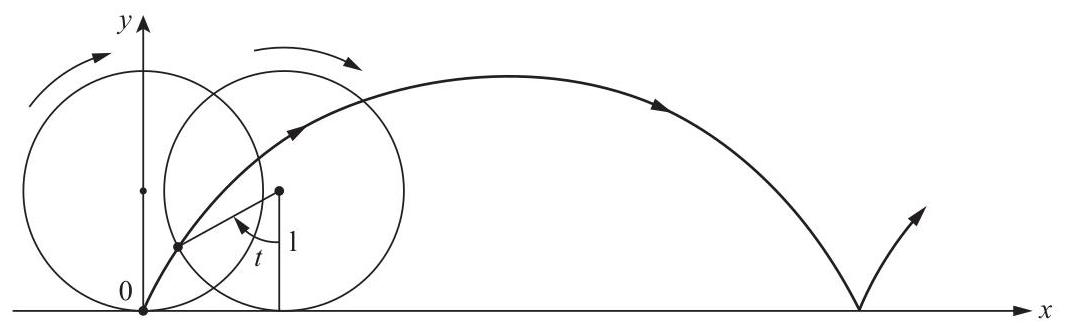
\includegraphics[max width=0.9\textwidth]{images/bo_d4b9jf3ef24c73e0334g_18_277_943_1065_326_0.jpg}
\captionof{figure}{图 1-7. 摆线.}
\end{center}

*a. 求一条轨迹为摆线的参数化曲线 $\alpha  : \mathbb{R} \rightarrow  \mathbb{R}^2$ ，并确定其奇异点.

b. 计算对应于圆盘完整旋转一周的摆线的弧长.
\begin{enumerate}
    \setcounter{enumi}{2}
    \item 令 $0A = 2a$ 为圆 $S^1$ 的直径， $0y$ 和 $AV$ 分别为 $S^1$ 在 0 和 $A$ 处的切线.从 0 画一条半直线 $r$ ，它与圆 $S^1$ 相交于 $C$ ，与直线 $AV$ 相交于 $B$ .在 $0B$ 上标出线段 $0p = CB$ .如果我们绕 0 旋转 $r$ ，点 $p$ 将描述一条称为迪奥克利斯蜗线的曲线.通过将 $0A$ 作为 $x$ 轴， $0Y$ 作为 $y$ 轴，证明:
\end{enumerate}
a. 痕迹

\[
\alpha(t)  = \left(\frac{2at^2}{1 + t^2},\frac{2at^3}{1 + t^2}\right) ,\;t \in  \mathbb{R},
\]

是迪奥克利斯蜗线( $t = \tan \theta$ ；见图 1-8).

b. 原点 $(0,0)$ 是蜗线的奇异点.

c. 当 $t \rightarrow  \infty ,\alpha(t)$ 趋近于直线 $x = 2a$ ，以及 $\alpha'(t)  \rightarrow  (0,2a)$ .因此，当 $t \rightarrow  \infty$ 时，曲线及其切线趋近于直线 $x = 2a$ ；我们称 $x = 2a$ 是蜗线的渐近线.
\begin{enumerate}
    \setcounter{enumi}{3}
    \item 令 $\alpha  : (0,\pi) \rightarrow  \mathbb{R}^2$ 由下式给出
    \[
    \alpha(t)  = (\sin t,\cos t + \log \tan \frac{t}{2}),
    \]
    其中 $t$ 是 $y$ 轴与向量 $\alpha'(t)$ 之间的夹角. $\alpha$ 的轨迹称为牵引线(图 1-9).证明:
\end{enumerate}

\begin{center}
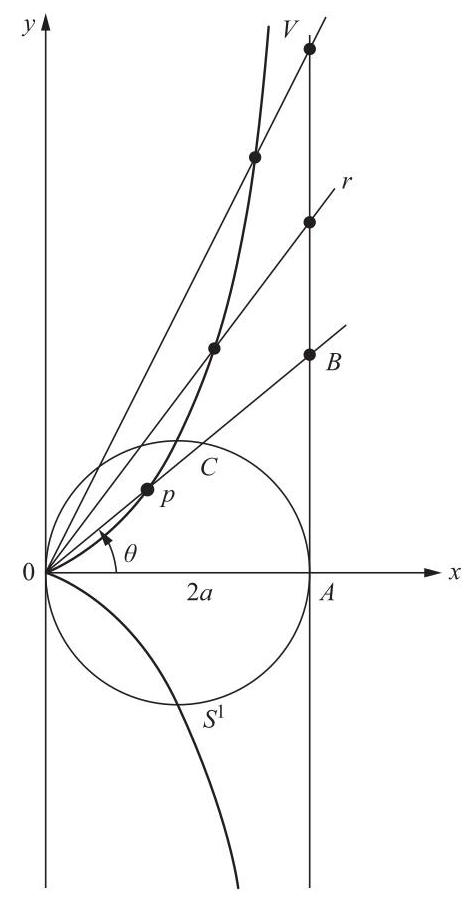
\includegraphics[max width=0.4\textwidth]{images/bo_d4b9jf3ef24c73e0334g_19_218_741_474_900_0.jpg}
\captionof{figure}{迪奥克利斯蜗线.}
\end{center}

\begin{center}
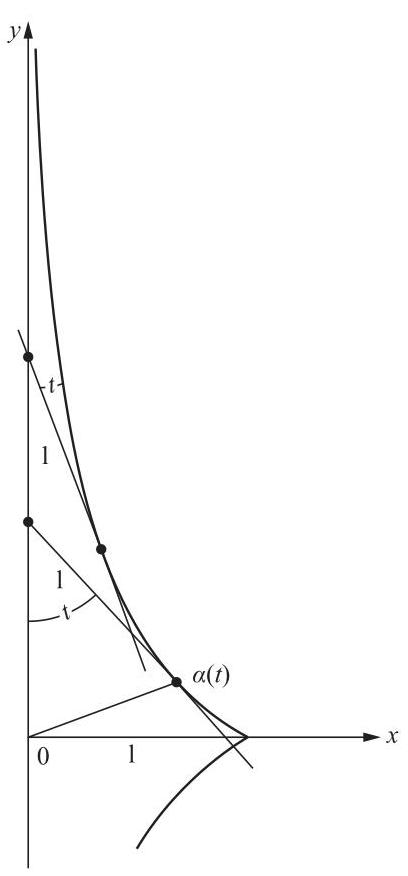
\includegraphics[max width=0.3\textwidth]{images/bo_d4b9jf3ef24c73e0334g_19_943_762_408_876_0.jpg}
\captionof{figure}{曳物线.}
\end{center}

a. $\alpha$ 是一个可微参数化曲线，在 $t = \pi /2$ 处不规则.

b. 曳物线上切线段在切点与 $y$ 轴之间的长度恒等于 1.
\begin{enumerate}
    \setcounter{enumi}{4}
    \item 令 $\alpha  : (-1, + \infty) \rightarrow  \mathbb{R}^2$ 由下式给出
    \[
    \alpha(t)  = \left(\frac{3at}{1 + t^3},\frac{3at^2}{1 + t^3}\right) .
    \]
\end{enumerate}
证明:

a. 对于 $t = 0,\alpha$ ，切线与 $x$ 轴相切.

b. 当 $t \rightarrow   + \infty ,\alpha(t)  \rightarrow  (0,0)$ 和 $\alpha'(t)  \rightarrow  (0,0)$ 时.

c. 取反向的曲线.现在，当 $t \rightarrow   - 1$ 时，曲线及其切线趋近于直线 $x + y + a = 0$ .

通过完成 $\alpha$ 的轨迹并使其相对于直线 $y = x$ 对称而得到的图形称为笛卡尔叶形线(见图 1-10).

\begin{center}
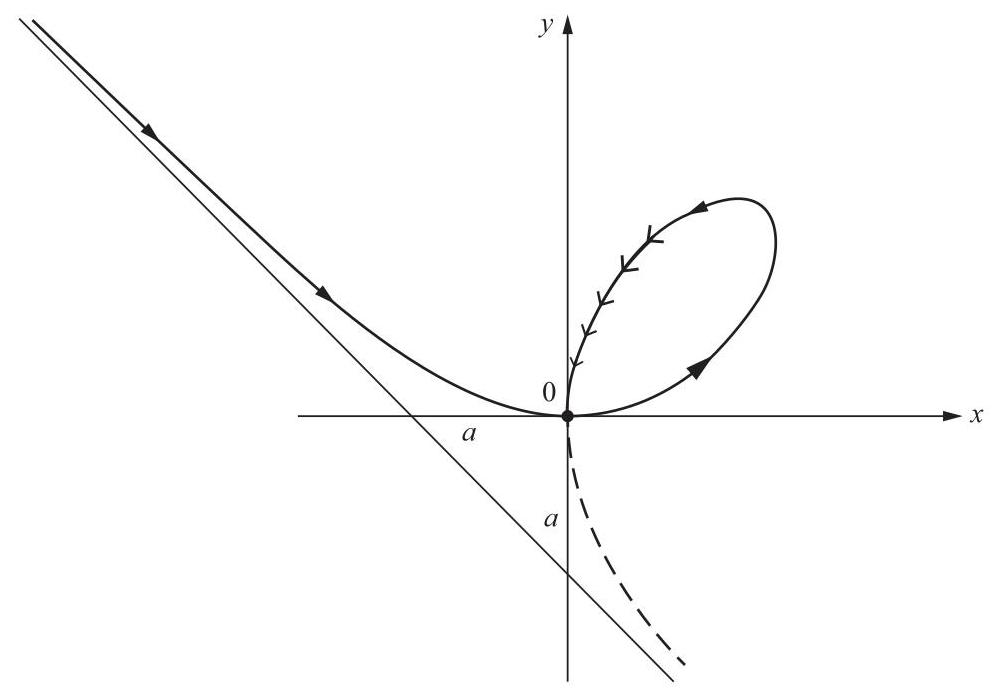
\includegraphics[max width=0.9\textwidth]{images/bo_d4b9jf3ef24c73e0334g_20_282_666_997_692_0.jpg}
\captionof{figure}{笛卡尔叶形线.}
\end{center}
\begin{enumerate}
    \setcounter{enumi}{5}
    \item 令 $\alpha(t)  = (ae^{bt}\cos t,ae^{bt}\sin t) ,t \in  \mathbb{R},a$ 和 $b$ 为常数， $a > 0$ ， $b < 0$ ，为参数化曲线.
\end{enumerate}
a. 证明当 $t \rightarrow   + \infty ,\alpha(t)$ 趋近于原点 0 时，围绕原点螺旋(因此， $\alpha$ 的轨迹称为对数螺线；见图 1-11).

b. 证明 $\alpha'(t)  \rightarrow  (0,0)$ 当 $t \rightarrow   + \infty$ 时，且

\[
\lim_{t \to +\infty} \int_{t_0}^{t} |\alpha'(t)| dt
\]

是有限的；也就是说， $\alpha$ 在 $[t_0,\infty)$ 中的弧长是有限的.

\begin{center}
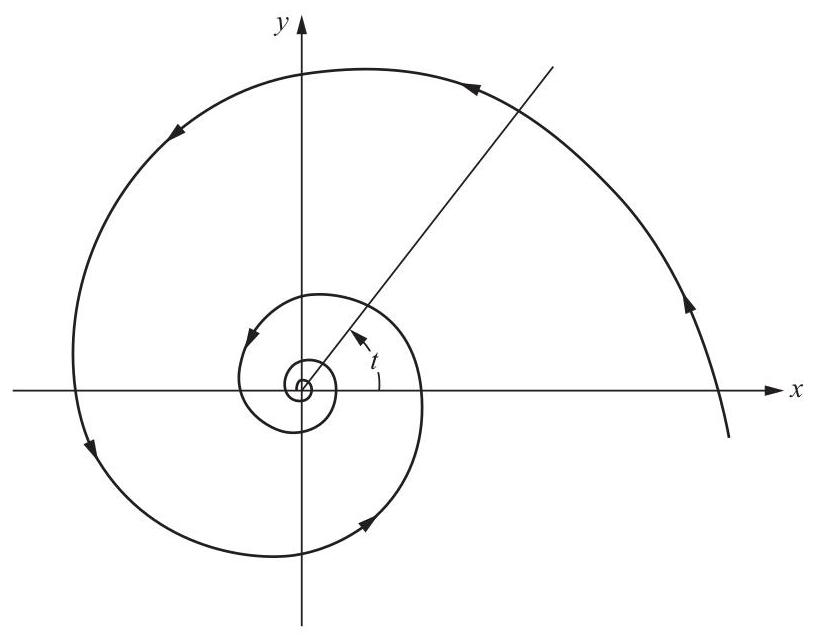
\includegraphics[max width=0.7\textwidth]{images/bo_d4b9jf3ef24c73e0334g_21_356_198_815_635_0.jpg}
\captionof{figure}{对数螺线.}
\end{center}
\begin{enumerate}
    \setcounter{enumi}{6}
    \item 映射 $\alpha  : I \rightarrow  \mathbb{R}^3$ 被称为 $C^k$ 类曲线，如果表达式 $\alpha(t)  = (x(t) ,y(t) ,z(t))$ 中每个坐标函数都具有直到 $k$ 阶的连续导数.如果 $\alpha$ 仅是连续的，则称 $\alpha$ 为 $C^0$ 类.曲线 $\alpha$ 被称为简单曲线，如果映射 $\alpha$ 是一一对应的.因此，1-2 节示例 3 中的曲线不是简单的.
\end{enumerate}
设 $\alpha  : I \rightarrow  \mathbb{R}^3$ 为一个 $C^0$ 类的简单曲线.当 $h \rightarrow  0$ 时，由 $\alpha(t_0 + h)$ 和 $\alpha(t_0)$ 确定的直线有极限位置，则称 $\alpha$ 在 $t = t_0 \in  I$ 处有弱切线.当 $h,k \rightarrow  0$ 时，由 $\alpha(t_0 + h)$ 和 $\alpha(t_0 + k)$ 确定的直线有极限位置，则称 $\alpha$ 在 $t = t_0$ 处有强切线.证明

a. $\alpha(t)  = (t^3,t^2) ,t \in  \mathbb{R}$ 在 $t = 0$ 处有弱切线但没有强切线.

*b. 如果 $\alpha  : I \rightarrow  \mathbb{R}^3$ 是 $C^1$ 类的且在 $t = t_0$ 处正则，则它在 $t = t_0$ 处有强切线.

c. 由以下给出的曲线

\[
\alpha(t)  = \begin{cases} (t^2,t^2), & t \geq  0, \\  (t^2, - t^2), & t \leq  0, \end{cases}
\]

是 $C^1$ 类的但不是 $C^2$ 类的.绘制曲线及其切向量的草图.
\begin{enumerate}
    \setcounter{enumi}{7}
    \item[*] 设 $\alpha  : I \rightarrow  \mathbb{R}^3$ 为一条可微曲线，设 $[a,b]   \subset  I$ 为一个闭区间.对于每一个划分
    \[
    a = t_0 < t_1 < \cdots  < t_n = b
    \]
    的 $[a,b]$ ，考虑和 $\sum_{i=1}^{n} |\alpha(t_i)  - \alpha(t_{i-1})|  = l(\alpha ,P)$ ，其中 $P$ 代表给定的划分.划分 $P$ 的范数 $|P|$ 定义为
    \[
    |P|  = \max(t_i - t_{i-1}) ,i = 1,\ldots ,n.
    \]
\end{enumerate}
几何上， $l(\alpha ,P)$ 是一个内接于 $\alpha([a,b])$ 且顶点在 $\alpha(t_i)$ 的多边形的长度(见图 1-12).本练习的目的是在某种意义上证明 $\alpha([a,b])$ 的弧长是内接多边形长度的极限.

\begin{center}
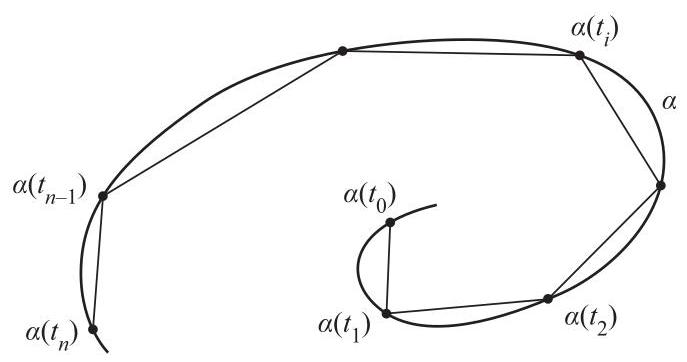
\includegraphics[max width=0.6\textwidth]{images/bo_d4b9jf3ef24c73e0334g_22_440_613_687_362_0.jpg}
\captionof{figure}{图 1-12}
\end{center}

证明对于给定的 $\varepsilon  > 0$ 存在 $\delta  > 0$ 使得如果 $|P|  < \delta$ 则

\[
\left| \int_{a}^{b} |\alpha'(t)| dt - l(\alpha ,P) \right|  < \varepsilon .
\]
\begin{enumerate}
    \setcounter{enumi}{8}
    \item 
    a. 设 $\alpha  : I \rightarrow  \mathbb{R}^3$ 为一个 $C^0$ 类的曲线(参见练习 7).使用练习 8 中描述的多边形近似法，给出弧长 $\alpha$ 的一个合理定义.
    b. (不可求长的曲线.) 下面的例子表明，对于任何合理的定义，闭区间内 $C^0$ 曲线的弧长可能是无界的.设 $\alpha  : [0,1]   \rightarrow  \mathbb{R}^2$ 定义为当 $t \neq  0$ 时 $\alpha(t)  = (t,t\sin(\pi /t))$ ，否则为 $\alpha(0)  = (0,0)$ .从几何上说明，对应于 $1/(n + 1)  \leq \; t \leq  1/n$ 的曲线部分的弧长至少为 $2/(n + \frac{1}{2})$ .利用这一点说明，区间 $1/N \leq  t \leq  1$ 内曲线的长度大于 $2\sum_{n=1}^{N} 1/(n + 1)$ ，因此当 $N \rightarrow  \infty$ 时，它趋于无穷大.
    \item (直线最短.) 设 $\alpha  : I \rightarrow  \mathbb{R}^3$ 为参数化曲线.设 $[a,b]   \subset  I$ 并令 $\alpha(a)  = p,\alpha(b)  = q$ .
\end{enumerate}
a. 证明，对于任何常向量 $v,|v|  = 1$ ，

\[
(q - p)  \cdot  v = \int_{a}^{b} \alpha'(t)  \cdot  v dt \leq  \int_{a}^{b} |\alpha'(t)| dt.
\]

b. 令

\[
v = \frac{q - p}{|q - p|}
\]

并证明

\[
|\alpha(b)  - \alpha(a)|  \leq  \int_{a}^{b} |\alpha'(t)| dt
\]

即，从 $\alpha(a)$ 到 $\alpha(b)$ 的最短曲线是连接这两点的直线.

\section{$\mathbb{R}^3$中的向量积}

在本节中，我们将介绍 $\mathbb{R}^3$ 中向量积的一些性质.这些性质将在我们后续研究曲线和曲面时非常有用.

为了方便起见，我们首先回顾向量空间的定向概念.一个 $n$ 维向量空间 $V$ 的两个有序基 $e = \{e_i\}$ 和 $f = \{f_i\}  ,i = 1,\ldots ,n$ 具有相同的定向，如果基变换矩阵的行列式为正.我们用 $e \sim  f$ 表示这种关系.从行列式的基本性质可知， $e \sim  f$ 是一个等价关系；即，它满足
\begin{enumerate}
    \item $e \sim  e$ .
    \item 如果 $e \sim  f$ ，则 $f \sim  e$ .
    \item 如果 $e \sim  f,f \sim  g$ ，则 $e \sim  g$ .
\end{enumerate}
因此， $V$ 的所有有序基的集合被分解为等价类(给定类中的元素通过 $\sim$ 相关联)，根据性质 3，这些等价类是不相交的.由于基变换的行列式要么为正，要么为负，因此这样的类只有两个.

由上述关系确定的每个等价类称为 $V$ 的一个定向.因此， $V$ 有两个定向，如果我们任意固定其中一个，另一个就称为相反的定向.

在 $V = \mathbb{R}^3$ 的情况下，存在一个自然的有序基 $e_1 = (1,0,0)$ ， $e_2 = (0,1,0) ,e_3 = (0,0,1)$ ，我们将对应于此基的定向称为 $\mathbb{R}^3$ 的正定向，另一个称为负定向(当然，这同样适用于任何 $\mathbb{R}^n$ ).我们也说一个给定的 $\mathbb{R}^3$ 的有序基是正的(或负的)，如果它属于 $\mathbb{R}^3$ 的正(或负)定向.因此，有序基 $e_1,e_3,e_2$ 是一个负基，因为将此基变换为 $e_1,e_2,e_3$ 的矩阵的行列式等于 -1.

现在我们来看向量积.设 $u,v \in  \mathbb{R}^3$ . $u$ 和 $v$ (按此顺序)的向量积是唯一的向量 $u \land  v \in  \mathbb{R}^3$ ，其特征为

\[
(u \land  v)  \cdot  w = \det(u,v,w) \;\text{ for all }w \in  \mathbb{R}^3.
\]

这里 $\det(u,v,w)$ 表示如果我们用自然基 $\{e_i\}$ 表示 $u,v$ 和 $w$ ，

\[
u = \sum u_ie_i,\;v = \sum v_ie_i
\]

\[
w = \sum w_ie_i,\;i = 1,2,3,
\]

那么

\[
\det(u,v,w)  = \begin{vmatrix} u_1 & u_2 & u_3 \\  v_1 & v_2 & v_3 \\  w_1 & w_2 & w_3 \end{vmatrix} ,
\]

其中 $|a_{ij}|$ 表示矩阵 $(a_{ij})$ 的行列式.从定义可以立即看出:

\[
u \land  v = \begin{vmatrix} u_2 & u_3 \\  v_2 & v_3 \end{vmatrix} e_1 - \begin{vmatrix} u_1 & u_3 \\  v_1 & v_3 \end{vmatrix} e_2 + \begin{vmatrix} u_1 & u_2 \\  v_1 & v_2 \end{vmatrix} e_3. \tag{1}
\]

注.也经常将 $u \land  v$ 写成 $u \times  v$ 并称之为叉积.

以下性质很容易验证(实际上它们只是表达了行列式的通常性质):
\begin{enumerate}
    \item $u \land  v =  - v \land  u$ (反对称性).
    \item $u \land  v$ 对 $u$ 和 $v$ 线性相关；即，对于任何实数 $a,b$ ，我们有
    \[
    (au + bw)  \land  v = au \land  v + bw \land  v.
    \]
    \item $u \land  v = 0$ 当且仅当 $u$ 和 $v$ 线性相关.
    \item $(u \land  v)  \cdot  u = 0,(u \land  v)  \cdot  v = 0$ .
\end{enumerate}
从性质 4 可以得出，向量积 $u \land  v \neq  0$ 与由 $u$ 和 $v$ 生成的平面正交.为了给出其范数和方向的几何解释，我们按如下方式进行.

首先，我们观察到 $(u \land  v)  \cdot  (u \land  v)  = |u \land  v|^2 > 0$ .这意味着向量 $u,v,u \land  v$ 的行列式为正；也就是说， $\{ u,v,u \land  v\}$ 是一个正基.

接下来，我们证明关系式

\[
(u \land  v)  \cdot  (x \land  y)  = \begin{vmatrix} u \cdot  x & v \cdot  x \\  u \cdot  y & v \cdot  y \end{vmatrix} ,
\]

其中 $u,v,x,y$ 是任意向量.这可以通过观察到两边都对 $u,v,x,y$ 线性来轻松完成.因此，只需检查:

\[
(e_i \land  e_j)  \cdot  (e_k \land  e_l)  = \begin{vmatrix} e_i \cdot  e_k & e_j \cdot  e_k \\  e_i \cdot  e_l & e_j \cdot  e_l \end{vmatrix}
\]

对于所有 $i,j,k,l = 1,2,3$ .这是一个直接的验证.

由此可知

\[
|u \land  v|^2 = \begin{vmatrix} u \cdot  u & u \cdot  v \\  u \cdot  v & v \cdot  v \end{vmatrix}  = |u|^2|v|^2(1 - \cos^2\theta)  = A^2,
\]

其中 $\theta$ 是 $u$ 和 $v$ 的角度， $A$ 是由 $u$ 和 $v$ 生成的平行四边形的面积.

简而言之， $u$ 和 $v$ 的向量积是一个向量 $u \land  v$ ，它垂直于由 $u$ 和 $v$ 张成的平面，其范数等于由 $u$ 和 $v$ 生成的平行四边形的面积，并且其方向使得 $\{ u,v,u \land  v\}$ 是一个正基(图 1-13).

\begin{center}
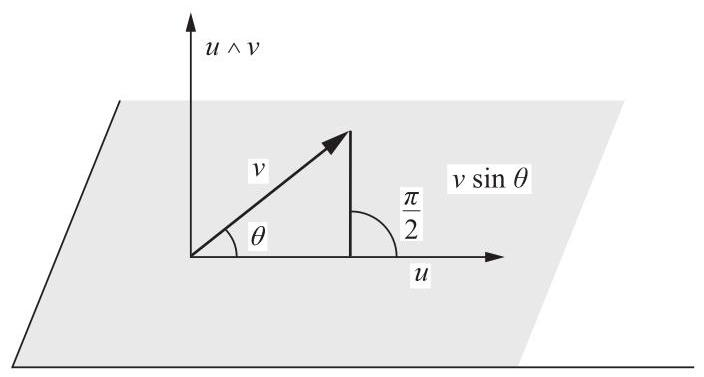
\includegraphics[max width=0.6\textwidth]{images/bo_d4b9jf3ef24c73e0334g_25_416_1282_704_377_0.jpg}
\captionof{figure}{图 1-13}
\end{center}

向量积不是结合律的.事实上，我们有以下恒等式:

\[
(u \land  v)  \land  w = (u \cdot  w) v - (v \cdot  w) u, \tag{2}
\]

这可以通过以下方式证明.首先我们注意到两边在 $u,v,w$ 上都是线性的；因此，如果恒等式对所有基向量都成立，那么它就是正确的.然而，最后的验证是直接的；例如，

\[
(e_1 \land  e_2)  \land  e_1 = e_2 = (e_1 \cdot  e_1) e_2 - (e_2 \cdot  e_1) e_1.
\]

最后，设 $u(t)  = (u_1(t) ,u_2(t) ,u_3(t))$ 和 $v(t)  = (v_1(t) ,v_2(t) ,v_3(t))$ 是从区间 $(a,b)$ 到 $\mathbb{R}^3,t \in  (a,b)$ 的可微映射.从公式 (1) 可以立即得出 $u(t)  \land  v(t)$ 也是可微的，并且

\[
\frac{d}{dt}(u(t)  \land  v(t))  = \frac{du}{dt} \land  v(t)  + u(t)  \land  \frac{dv}{dt}.
\]

向量积在许多几何构造中自然出现.实际上， $\mathbb{R}^3$ 中平面和直线的绝大多数几何性质都可以用向量积和行列式来简洁地表达.我们将在接下来的练习中回顾其中一些材料.

\exerciseline
\begin{enumerate}
    \item 检查以下基是否为正基:
\begin{enumerate}
    \item[a.] $\mathbb{R}^2$ 中的基 $\{ (1,3) ,(4,2) \}$ .
    \item[b.] $\mathbb{R}^3$ 中的基 $\{ (1,3,5) ,(2,3,7) ,(4,8,3) \}$ .
\end{enumerate}
    \item[*] 给定一个包含在 $\mathbb{R}^3$ 中的平面 $P$ ，其方程为 $ax + by + cz + d = 0$ .证明向量 $v = (a,b,c)$ 垂直于该平面，并且 $|d| /\sqrt{a^2 + b^2 + c^2}$ 度量了从该平面到原点 $(0,0,0)$ 的距离.
    \item[*] 确定两个平面 $5x + 3y +  2z - 4 = 0$ 和 $3x + 4y - 7z = 0$ 的交角.
    \item[*] 给定两个平面 $a_ix + b_iy + c_iz + d_i = 0,i = 1,2$ ，证明它们平行的充要条件是
    \[
    \frac{a_1}{a_2} = \frac{b_1}{b_2} = \frac{c_1}{c_2}
    \]
    其中约定，若分母为零，则对应的分子也为零(当两个平面重合或不相交时，我们称它们平行).
    \item 证明通过三个非共点 $p_1 = (x_1,y_1,z_1) ,p_2 = (x_2,y_2,z_2) ,p_3 = (x_3,y_3,z_3)$ 的平面方程为
    \[
    (p - p_1)  \land  (p - p_2)  \cdot  (p - p_3)  = 0,
    \]
\end{enumerate}

其中 \(p = \left( {x,y,z}\right)\) 是平面上的任意一点，而 \(p - {p}_{1}\) 例如表示向量 \(\left( {x - {x}_{1},y - {y}_{1},z - {z}_{1}}\right)\) .

*6. 给定两个非平行平面 \({a}_{i}x + {b}_{i}y + {c}_{i}z + {d}_{i} = 0,i = 1,2\) ，证明它们的交线可参数化为

\[
x - {x}_{0} = {u}_{1}t,\;y - {y}_{0} = {u}_{2}t,\;z - {z}_{0} = {u}_{3}t,
\]

其中 \(\left( {{x}_{0},{y}_{0},{z}_{0}}\right)\) 属于交集，而 \(u = \left( {{u}_{1},{u}_{2},{u}_{3}}\right)\) 是向量积 \(u = {v}_{1} \land  {v}_{2},{v}_{i} = \left( {{a}_{i},{b}_{i},{c}_{i}}\right) ,i = 1,2\) .

*7. 证明平面

\[
{ax} + {by} + {cz} + d = 0
\]

与直线 \(x - {x}_{0} = {u}_{1}t,y - {y}_{0} = {u}_{2}t,z - {z}_{0} = {u}_{3}t\) 平行的充要条件是

\[
a{u}_{1} + b{u}_{2} + c{u}_{3} = 0.
\]

*8. 证明非平行线之间的距离 \(\rho\) 为

\[
x - {x}_{0} = {u}_{1}t,\;y - {y}_{0} = {u}_{2}t,\;z - {z}_{0} = {u}_{3}t,
\]

\[
x - {x}_{1} = {v}_{1}t,\;y - {y}_{1} = {v}_{2}t,\;z - {z}_{1} = {v}_{3}t
\]

由下式给出

\[
\rho  = \frac{\left| \left( u \land  v\right)  \cdot  r\right| }{\left| u \land  v\right| }
\]

其中 \(u = \left( {{u}_{1},{u}_{2},{u}_{3}}\right) ,v = \left( {{v}_{1},{v}_{2},{v}_{3}}\right) ,r = \left( {{x}_{0} - {x}_{1},{y}_{0} - {y}_{1},{z}_{0} - {z}_{1}}\right)\) .

9. 求平面 \({3x} + {4y} + {7z} + 8 = 0\) 与直线 \(x - 2 = {3t},y - 3 = {5t},z - 5 = {9t}\) 的交角.

10. \({R}^{2}\) 的自然定向使得我们可以为由两个线性无关向量 \(u,v \in  {R}^{2}\) 生成的平行四边形 \(A\) 的面积赋予符号.为此，设 \(\left\{  {e}_{i}\right\}  ,i = 1,2\) 为 \({R}^{2}\) 的自然有序基，并写出 \(u = {u}_{1}{e}_{1} + {u}_{2}{e}_{2},v = {v}_{1}{e}_{1} + {v}_{2}{e}_{2}\) .观察矩阵关系

\[
\left( \begin{array}{ll} u \cdot  u & u \cdot  v \\  v \cdot  u & v \cdot  v \end{array}\right)  = \left( \begin{array}{ll} {u}_{1} & {u}_{2} \\  {v}_{1} & {v}_{2} \end{array}\right) \left( \begin{array}{ll} {u}_{1} & {v}_{1} \\  {u}_{2} & {v}_{2} \end{array}\right)
\]

并得出

\[
{A}^{2} = {\left| \begin{array}{ll} {u}_{1} & {u}_{2} \\  {v}_{1} & {v}_{2} \end{array}\right| }^{2}
\]

由于最后一个行列式与基 \(\{ u,v\}\) 同号，我们可以说 \(A\) 为正或负，取决于 \(\{ u,v\}\) 的定向是正还是负.这称为 \({R}^{2}\) 中的定向面积.

11. a. 证明由三个线性无关向量 \(u,v,w \in  {R}^{3}\) 生成的平行六面体的体积 \(V\) 由 \(V = \left| {\left( {u \land  v}\right)  \cdot  w}\right|\) 给出，并在 \({R}^{3}\) 中引入定向体积.

b. 证明

\[
{V}^{2} = \left| \begin{matrix} u \cdot  u & u \cdot  v & u \cdot  w \\  v \cdot  u & v \cdot  v & v \cdot  w \\  w \cdot  u & w \cdot  v & w \cdot  w \end{matrix}\right| .
\]

12. 给定向量 \(v \neq  0\) 和 \(w\) ，证明存在向量 \(u\) 使得 \(u \land  v = w\) 当且仅当 \(v\) 垂直于 \(w\) .该向量 \(u\) 是否唯一确定？如果不是，最一般的解是什么？

13. 令 \(u\left( t\right)  = \left( {{u}_{1}\left( t\right) ,{u}_{2}\left( t\right) ,{u}_{3}\left( t\right) }\right)\) 和 \(v\left( t\right)  = \left( {{v}_{1}\left( t\right) ,{v}_{2}\left( t\right) ,{v}_{3}\left( t\right) }\right)\) 为从区间 \(\left( {a,b}\right)\) 到 \({R}^{3}\) 的可微映射.如果导数 \({u}^{\prime }\left( t\right)\) 和 \({v}^{\prime }\left( t\right)\) 满足条件

\[
{u}^{\prime }\left( t\right)  = {au}\left( t\right)  + {bv}\left( t\right) ,\;{v}^{\prime }\left( t\right)  = {cu}\left( t\right)  - {av}\left( t\right) ,
\]

其中 \(a,b\) 和 \(c\) 是常数，证明 \(u\left( t\right)  \land  v\left( t\right)\) 是一个常向量.

14. 求所有单位向量，它们垂直于向量 \(\left( {2,2,1}\right)\) 且平行于由点 \(\left( {0,0,0}\right) ,\left( {1, - 2,1}\right)\) 、 \(\left( {-1,1,1}\right)\) 确定的平面.

\section{由弧长参数化的曲线的局部理论}

本节包含本书后续部分将使用的曲线的主要结果.

令 \(\alpha  : I = \left( {a,b}\right)  \rightarrow  {R}^{3}\) 为由弧长 \(s\) 参数化的曲线.由于切向量 \({\alpha }^{\prime }\left( s\right)\) 的长度为单位长度，二阶导数的范数 \(\left| {{\alpha }^{\prime \prime }\left( s\right) }\right|\) 度量了邻近切线与 \(s.\left| {{\alpha }^{\prime \prime }\left( s\right) }\right|\) 处的切线所成的角度的变化率，因此，它度量了曲线在 \(s\) 的邻域内离开切线 \(s\) 的速度(见图 1-14).这提示了以下定义.

定义.令 \(\alpha  : \mathrm{I} \rightarrow  {\mathbb{R}}^{3}\) 为由弧长 \(\mathrm{s} \in  \mathrm{I}\) 参数化的曲线.数 \(\left| {{\alpha }^{\prime \prime }\left( \mathrm{s}\right) }\right|  = \mathrm{k}\left( \mathrm{s}\right)\) 被称为 \(\alpha\) 在 \(\mathrm{s}\) 处的曲率.

如果 \(\alpha\) 是一条直线， \(\alpha \left( s\right)  = {us} + v\) ，其中 \(u\) 和 \(v\) 是常向量 \(\left( {\left| u\right|  = 1}\right)\) ，则 \(k \equiv  0\) .反之，如果 \(k = \left| {{\alpha }^{\prime \prime }\left( s\right) }\right|  \equiv  0\) ，则通过积分 \(\alpha \left( s\right)  = {us} + v\) ，曲线是一条直线.

\begin{center}
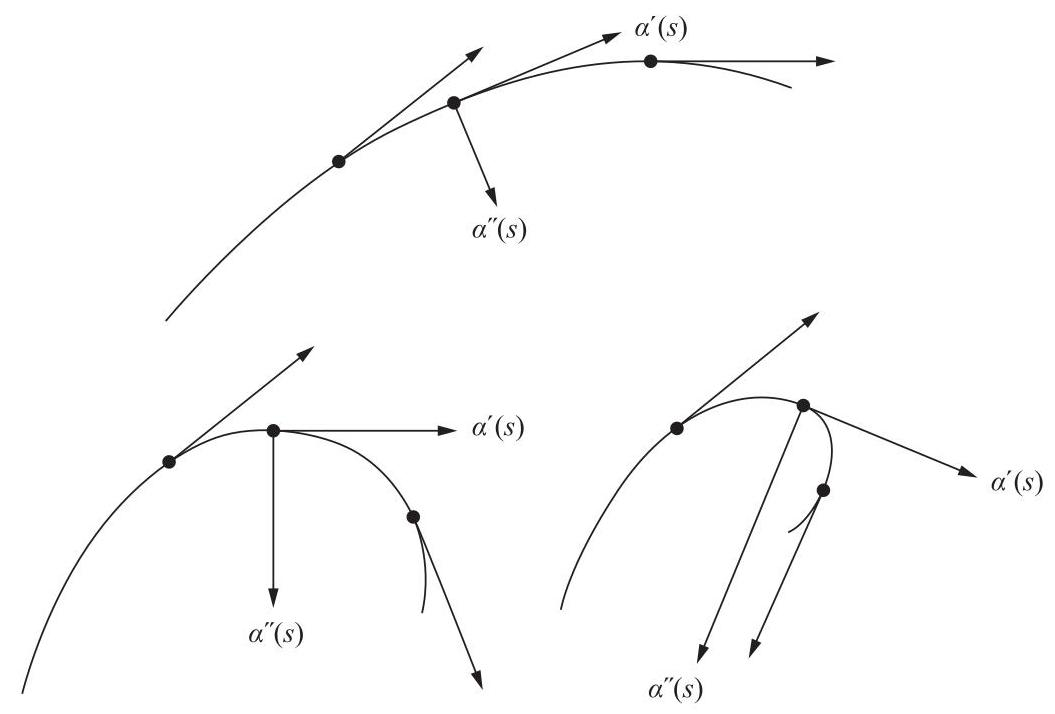
\includegraphics[max width=0.9\textwidth]{images/bo_d4b9jf3ef24c73e0334g_29_230_194_1055_714_0.jpg}
\end{center}
\hspace*{3em} 

图 1-14

注意，通过改变方向，切向量改变其方向；也就是说，如果 \(\beta \left( {-s}\right)  = \alpha \left( s\right)\) ，则

\[
\frac{d\beta }{d\left( {-s}\right) }\left( {-s}\right)  =  - \frac{d\alpha }{ds}\left( s\right) .
\]

因此， \({\alpha }^{\prime \prime }\left( s\right)\) 和曲率在方向改变下保持不变.

在 \(k\left( s\right)  \neq  0\) 的点处，方向 \({\alpha }^{\prime \prime }\left( s\right)\) 上的单位向量 \(n\left( s\right)\) 由方程 \({\alpha }^{\prime \prime }\left( s\right)  = k\left( s\right) n\left( s\right)\) 明确定义.此外， \({\alpha }^{\prime \prime }\left( s\right)\) 垂直于 \({\alpha }^{\prime }\left( s\right)\) ，因为通过对 \({\alpha }^{\prime }\left( s\right)  \cdot  {\alpha }^{\prime }\left( s\right)  = 1\) 求导，我们得到 \({\alpha }^{\prime \prime }\left( s\right)  \cdot  {\alpha }^{\prime }\left( s\right)  = 0\) .因此， \(n\left( s\right)\) 垂直于 \({\alpha }^{\prime }\left( s\right)\) ，并称为 \(s\) 处的法向量.由单位切向量和法向量 \({\alpha }^{\prime }\left( s\right)\) 和 \(n\left( s\right)\) 确定的平面称为 \(s\) 处的密切平面.(参见图 1-15.)

在 \(k\left( s\right)  = 0\) 的点处，法向量(因此密切平面)未定义(参见练习 10).为了继续对曲线进行局部分析，我们本质上需要密切平面.因此，方便地说，如果 \({\alpha }^{\prime \prime }\left( s\right)  = 0\) (在此上下文中， \({\alpha }^{\prime }\left( s\right)  = 0\) 的点称为零阶奇异点)，则 \(s \in  I\) 是一个一阶奇异点.

在下文中，我们将仅限于由弧长参数化且没有一阶奇异点的曲线.我们将用 \(t\left( s\right)  = {\alpha }^{\prime }\left( s\right)\) 表示 \(\alpha\) 在 \(s\) 处的单位切向量.因此， \({t}^{\prime }\left( s\right)  = k\left( s\right) n\left( s\right)\) .

单位向量 \(b\left( s\right)  = t\left( s\right)  \land  n\left( s\right)\) 垂直于密切平面，并将被称为 \(s\) 处的副法向量.由于 \(b\left( s\right)\) 是单位向量，长度 \(\left| {{b}^{\prime }\left( s\right) }\right|\) 度量了邻近密切平面相对于 \(s\) 处的密切平面的变化率；也就是说， \(\left| {{b}^{\prime }\left( s\right) }\right|\) 度量了曲线在 \(s\) 的邻域中离开 \(s\) 处的密切平面的速度(参见图 1-15).

\begin{center}
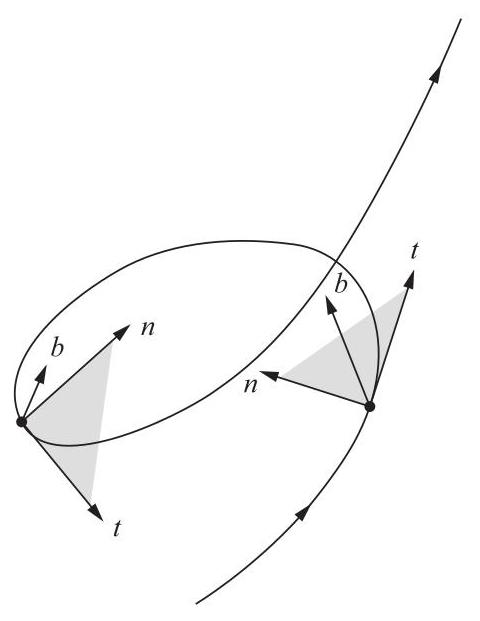
\includegraphics[max width=0.4\textwidth]{images/bo_d4b9jf3ef24c73e0334g_30_195_187_480_621_0.jpg}
\end{center}
\hspace*{3em} 

图 1-15

为了计算 \({b}^{\prime }\left( s\right)\) ，我们注意到一方面 \({b}^{\prime }\left( s\right)\) 垂直于 \(b\left( s\right)\) ，另一方面，

\[
{b}^{\prime }\left( s\right)  = {t}^{\prime }\left( s\right)  \land  n\left( s\right)  + t\left( s\right)  \land  {n}^{\prime }\left( s\right)  = t\left( s\right)  \land  {n}^{\prime }\left( s\right) ;
\]

也就是说， \({b}^{\prime }\left( s\right)\) 垂直于 \(t\left( s\right)\) .因此， \({b}^{\prime }\left( s\right)\) 平行于 \(n\left( s\right)\) ，我们可以写成

\[
{b}^{\prime }\left( s\right)  = \tau \left( s\right) n\left( s\right)
\]

对于某个函数 \(\tau \left( s\right)\) .(警告:许多作者使用 \(- \tau \left( s\right)\) 而不是我们的 \(\tau \left( s\right)\) .)

定义. 设 \(\alpha  : \mathrm{I} \rightarrow  {\mathbb{R}}^{3}\) 为一由弧长 \(\mathrm{s}\) 参数化的曲线，使得 \({\alpha }^{\prime \prime }\left( \mathrm{s}\right)  \neq  0,\mathrm{\;s} \in  \mathrm{I}\) . 由 \({\mathrm{b}}^{\prime }\left( \mathrm{s}\right)  = \tau \left( \mathrm{s}\right) \mathrm{n}\left( \mathrm{s}\right)\) 定义的数 \(\tau \left( \mathrm{s}\right)\) 称为 \(\alpha\) 在 \(\mathrm{s}\) 处的挠率.

如果 \(\alpha\) 是平面曲线(即 \(\alpha \left( I\right)\) 包含于一个平面内)，则曲线的平面与密切平面一致；因此， \(\tau  \equiv  0\) . 反之，如果 \(\tau  \equiv  0\) (且 \(k \neq  0\) )，我们有 \(b\left( s\right)  = {b}_{0} =\) 为常数，因此

\[
{\left( \alpha \left( s\right)  \cdot  {b}_{0}\right) }^{\prime } = {\alpha }^{\prime }\left( s\right)  \cdot  {b}_{0} = 0.
\]

由此可知 \(\alpha \left( s\right)  \cdot  {b}_{0} =\) 为常数；因此， \(\alpha \left( s\right)\) 包含于一个垂直于 \({b}_{0}\) 的平面内. \(k \neq  0\) 处处成立的条件在此是必不可少的. 在练习 10 中，我们将给出一个例子，其中 \(\tau\) 可以定义为恒等于零，但曲线却不是平面曲线.

与曲率不同，挠率可以是正的或负的. 挠率的符号具有几何意义，将在后面给出(第 1-6 节).

注意到通过改变方向，副法线向量改变符号，因为 \(b = t \land  n\) . 因此， \({b}^{\prime }\left( s\right)\) ，从而挠率，在改变方向下保持不变.

总结我们的立场. 对于参数 \(s\) 的每个值，我们都关联了三个正交单位向量 \(t\left( s\right) ,n\left( s\right) ,b\left( s\right)\) . 这样形成的坐标系称为 \(s\) 处的弗雷内坐标系. 向量 \(t\left( s\right)\) 和 \(b\left( s\right)\) 的导数 \({t}^{\prime }\left( s\right)  = {kn}\) 和 \({b}^{\prime }\left( s\right)  = {\tau n}\) ，当用基 \(\{ t,n,b\}\) 表示时，产生了几何实体(曲率 \(k\) 和挠率 \(\tau\) )，它们提供了关于 \(\alpha\) 在 \(s\) 邻域行为的信息.

寻找其他局部几何实体将引导我们计算 \({n}^{\prime }\left( s\right)\) . 然而，由于 \(n = b \land  t\) ，我们有

\[
{n}^{\prime }\left( s\right)  = {b}^{\prime }\left( s\right)  \land  t\left( s\right)  + b\left( s\right)  \land  {t}^{\prime }\left( s\right)  =  - {\tau b} - {kt},
\]

我们再次得到曲率和挠率.

为了以后使用，我们将方程

\[
{t}^{\prime } = {kn}
\]

\[
{n}^{\prime } =  - {kt} - {\tau b},
\]

\[
{b}^{\prime } = {\tau n}
\]

称为弗雷内公式(为方便起见，我们省略了 \(s\) ). 在此上下文中，以下术语是常用的. \({tb}\) 平面称为切法平面， \({nb}\) 平面称为法平面. 通过 \(\alpha \left( s\right)\) 且包含 \(n\left( s\right)\) 和 \(b\left( s\right)\) 的直线分别称为主法线和副法线. 曲率的倒数 \(R = 1/k\) 称为 \(s\) 处的曲率半径. 当然，半径为 \(r\) 的圆的曲率半径等于 \(r\) ，正如可以轻易验证的那样.

从物理上讲，我们可以将 \({R}^{3}\) 中的曲线视为由直线通过弯曲(曲率)和扭曲(挠率)得到. 反思这个构造后，我们推测以下陈述，该陈述大致表明 \(k\) 和 \(\tau\) 完全描述了曲线的局部行为.

曲线局部理论基本定理.给定可微函数 \(\mathrm{k}\left( \mathrm{s}\right)  > 0\) 和 \(\tau \left( \mathrm{s}\right) ,\mathrm{s} \in  \mathrm{I}\) ，存在一条正则参数化曲线 \(\alpha  : \mathrm{I} \rightarrow  {\mathbb{R}}^{3}\) ，使得 \(\mathrm{s}\) 是其弧长， \(\mathrm{k}\left( \mathrm{s}\right)\) 是其曲率， \(\tau \left( \mathrm{s}\right)\) 是其挠率.此外，任何其他满足相同条件的曲线 \(\overline{\alpha }\) ，与 \(\alpha\) 仅相差一个刚体运动；也就是说，存在一个 \({\mathbb{R}}^{3}\) 的正定交替线性映射 \(\rho\) 和一个向量 \(\mathrm{c}\) ，使得 \(\overline{\alpha } = \rho  \circ  \alpha  + \mathrm{c}\) .

上述陈述是正确的.完整的证明涉及常微分方程解的存在唯一性定理，将在第 4 章的附录中给出.然而，具有相同 \(s,k\left( s\right)\) 和 \(\tau \left( s\right)\) 的曲线，在刚体运动下的唯一性证明很简单，可以在这里给出.

基本定理唯一性部分的证明.我们首先注意到，弧长、曲率和挠率在刚体运动下是不变的；这意味着，例如，如果 \(M : {R}^{3} \rightarrow  {R}^{3}\) 是一个刚体运动，而 \(\alpha  = \alpha \left( t\right)\) 是一条参数化曲线，那么

\[
{\int }_{a}^{b}\left| \frac{d\alpha }{dt}\right| {dt} = {\int }_{a}^{b}\left| \frac{d\left( {M \circ  \alpha }\right) }{dt}\right| {dt}.
\]

这是合理的，因为这些概念是通过使用某些导数的内积或向量积来定义的(导数在平移下不变，而内积和向量积通过向量的长度和角度来表示，因此在刚体运动下也不变).仔细的验证可以留作练习(参见练习 6).

现在，假设两条曲线 \(\alpha  = \alpha \left( s\right)\) 和 \(\overline{\alpha } = \overline{\alpha }\left( s\right)\) 满足条件 \(k\left( s\right)  = \bar{k}\left( s\right)\) 和 \(\tau \left( s\right)  = \overline{\tau }\left( s\right) ,s \in  I\) .令 \({t}_{0},{n}_{0},{b}_{0}\) 和 \({\bar{t}}_{0},{\bar{n}}_{0},{\bar{b}}_{0}\) 分别为 \(\alpha\) 和 \(\overline{\alpha }\) 在 \(s = {s}_{0} \in  I\) 处的弗雷内标架.显然，存在一个刚体运动，可以将 \(\overline{\alpha }\left( {s}_{0}\right)\) 映射到 \(\alpha \left( {s}_{0}\right)\) ，并将 \({\bar{t}}_{0},{\bar{n}}_{0},{\bar{b}}_{0}\) 映射到 \({t}_{0},{n}_{0},{b}_{0}\) .因此，在对 \(\overline{\alpha }\) 执行此刚体运动后，我们得到 \(\overline{\alpha }\left( {s}_{0}\right)  = \alpha \left( {s}_{0}\right)\) ，并且 \(\alpha\) 和 \(\overline{\alpha }\) 的弗雷内标架 \(t\left( s\right) ,n\left( s\right) ,b\left( s\right)\) 和 \(\bar{t}\left( s\right) ,\bar{n}\left( s\right) ,\bar{b}\left( s\right)\) 分别满足弗雷内方程:

\[
\frac{dt}{ds} = {kn}\;\frac{d\bar{t}}{ds} = k\bar{n}
\]

\[
\frac{dn}{ds} =  - {kt} - {\tau b}\;\frac{d\bar{n}}{ds} =  - k\bar{t} - \tau \bar{n}
\]

\[
\frac{db}{ds} = {\tau n}\;\frac{d\bar{b}}{ds} = \tau \bar{n}
\]

与 \(t\left( {s}_{0}\right)  = \bar{t}\left( {s}_{0}\right) ,n\left( {s}_{0}\right)  = \bar{n}\left( {s}_{0}\right) ,b\left( {s}_{0}\right)  = \bar{b}\left( {s}_{0}\right)\) .

我们现在通过使用弗莱纳方程观察到，

\[
\frac{1}{2}\frac{d}{ds}\left\{  {{\left| t - \bar{t}\right| }^{2} + {\left| n - \bar{n}\right| }^{2} + {\left| b - \bar{b}\right| }^{2}}\right\}
\]

\[
= \left\langle  {t - \bar{t},{t}^{\prime } - {\bar{t}}^{\prime }}\right\rangle   + \left\langle  {b - \bar{b},{b}^{\prime } - {\bar{b}}^{\prime }}\right\rangle   + \left\langle  {n - \bar{n},{n}^{\prime } - {\bar{n}}^{\prime }}\right\rangle
\]

\[
= k\langle t - \bar{t},n - \bar{n}\rangle  + \tau \langle b - \bar{b},n - \bar{n}\rangle  - k\langle n - \bar{n},t - \bar{t}\rangle
\]

\[
- \tau \langle n - \bar{n},b - \bar{b}\rangle
\]

\[
= 0
\]

对于所有 \(s \in  I\) .因此，上述表达式是常数，并且由于它对于 \(s = {s}_{0}\) 为零，所以它恒为零.由此可知，对于所有 \(s \in  I\) ，都有 \(t\left( s\right)  = \bar{t}\left( s\right) ,n\left( s\right)  = \bar{n}\left( s\right) ,b\left( s\right)  = \; \bar{b}\left( s\right)\) .因为

\[
\frac{d\alpha }{ds} = t = \bar{t} = \frac{d\overline{\alpha }}{ds},
\]

我们得到 \(\left( {d/{ds}}\right) \left( {\alpha  - \overline{\alpha }}\right)  = 0\) .因此， \(\alpha \left( s\right)  = \overline{\alpha }\left( s\right)  + a\) ，其中 \(a\) 是一个常向量.因为 \(\alpha \left( {s}_{0}\right)  = \overline{\alpha }\left( {s}_{0}\right)\) ，我们有 \(a = 0\) ；因此，对于所有 \(s \in  I\) ，都有 \(\alpha \left( s\right)  = \overline{\alpha }\left( s\right)\) .

Q.E.D.

注1.在平面曲线 \(\alpha  : I \rightarrow  {R}^{2}\) 的特例中，可以给曲率 \(k\) 规定一个符号.为此，设 \(\left\{  {{e}_{1},{e}_{2}}\right\}\) 为 \({R}^{2}\) 的自然基(见第1-4节)，并定义法向量 \(n\left( s\right) ,s \in  I\) ，要求基 \(\{ t\left( s\right) ,n\left( s\right) \}\) 与基 \(\left\{  {{e}_{1},{e}_{2}}\right\}\) 具有相同的方向.然后定义曲率 \(k\) 为

\[
\frac{dt}{ds} = {kn}
\]

并且可以是正的或负的.显然， \(\left| k\right|\) 与之前的定义一致，并且当改变 \(\alpha\) 的方向或 \({R}^{2}\) 的方向时， \(k\) 会改变符号(图1-16).

\begin{center}
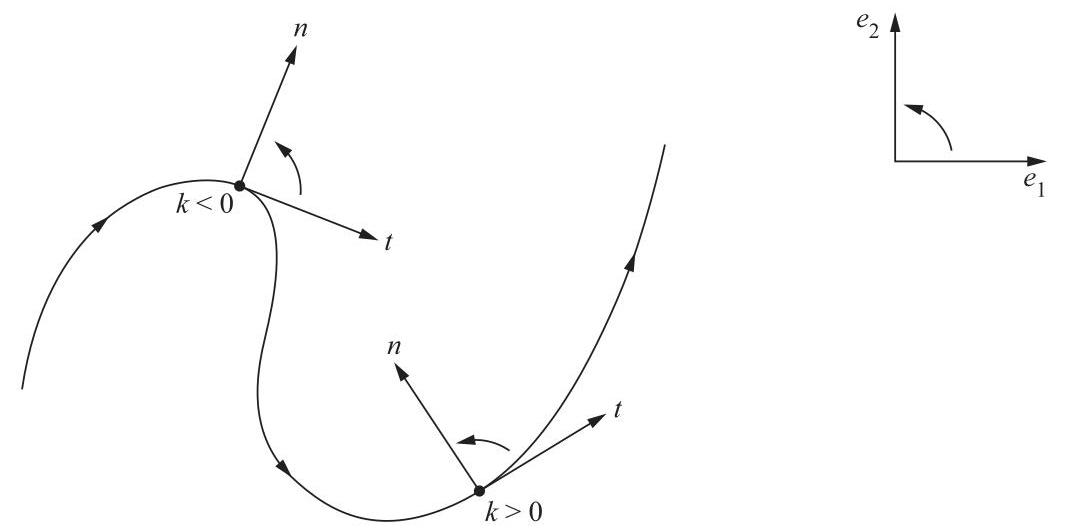
\includegraphics[max width=0.9\textwidth]{images/bo_d4b9jf3ef24c73e0334g_33_232_1002_1065_532_0.jpg}
\end{center}
\hspace*{3em} 

图1-16

还应该指出的是，在平面曲线 \(\left( {\tau  \equiv  0}\right)\) 的情况下，上述基本定理的证明实际上非常简单(见练习9).

注2.给定一条正则参数化曲线 \(\alpha  : I \rightarrow  {R}^{3}\) (不一定是弧长参数化)，可以得到一条参数化曲线 \(\beta  : J \rightarrow  {R}^{3}\) ，它具有与 \(\alpha\) 相同的轨迹.事实上，设

\[
s = s\left( t\right)  = {\int }_{{t}_{0}}^{t}\left| {{\alpha }^{\prime }\left( t\right) }\right| {dt},\;t,{t}_{0} \in  I.
\]

因为 \({ds}/{dt} = \left| {{\alpha }^{\prime }\left( t\right) }\right|  \neq  0\) ，函数 \(s = s\left( t\right)\) 有一个可微的逆函数 \(t = t\left( s\right) ,s \in  s\left( I\right)  = J\) ，其中，通过滥用符号， \(t\) 也表示 \(s\) 的逆函数 \({s}^{-1}\) .现在设 \(\beta  = \alpha  \circ  t : J \rightarrow  {R}^{3}\) .显然， \(\beta \left( J\right)  = \alpha \left( I\right)\) 和 \(\left| {{\beta }^{\prime }\left( s\right) }\right|  = \left| {({\alpha }^{\prime }\left( t\right)  \cdot  \left( {{dt}/{ds}}\right) }\right|  = 1\) .这表明 \(\beta\) 与 \(\alpha\) 具有相同的轨迹，并且是弧长参数化的.通常说 \(\beta\) 是 \(\alpha \left( I\right)\) 的弧长重参数化.

这一事实允许我们将先前定义的所有局部概念推广到具有任意参数的正則曲線.因此，我们说 \(\alpha  : I \rightarrow  {R}^{3}\) 在 \(t \in  I\) 处的曲率 \(k\left( t\right)\) 是通过弧长对 \(\alpha \left( I\right)\) 的重参数化 \(\beta  : J \rightarrow  {R}^{3}\) 在相应点 \(s = s\left( t\right)\) 处的曲率.这显然与 \(\beta\) 的选择无关，并表明在第 1-3 节末尾所做的仅考虑由弧长参数化的曲线的限制并非本质性的.

在应用中，通常方便地获得任意参数的几何实体的显式公式；我们将在练习 12 中给出其中一些.

\exerciseline

除非另有明确说明， \(\alpha  : \mathrm{I} \rightarrow  {\mathbb{R}}^{3}\) 是由弧长 \(\mathrm{s}\) 参数化的曲线，其曲率 \(\mathrm{k}\left( \mathrm{s}\right)  \neq  0\) 对所有 \(\mathrm{s} \in  \mathrm{I}\) 成立.

1. 给定参数化曲线(螺旋线)

\[
\alpha \left( s\right)  = \left( {a\cos \frac{s}{c},a\sin \frac{s}{c},b\frac{s}{c}}\right) ,\;s \in  R,
\]

其中 \({c}^{2} = {a}^{2} + {b}^{2}\) ，

a. 证明参数 \(s\) 是弧长.

b. 确定 \(\alpha\) 的曲率和挠率.

c. 确定 \(\alpha\) 的密切平面.

d. 证明包含 \(n\left( s\right)\) 并通过 \(\alpha \left( s\right)\) 的直线与 \(z\) 轴相交的角度恒定，等于 \(\pi /2\) .

e. 证明 \(\alpha\) 的切线与 \(z\) 轴成恒定角度.

*2. 证明 \(\alpha\) 的挠率 \(\tau\) 由下式给出

\[
\tau \left( s\right)  =  - \frac{{\alpha }^{\prime }\left( s\right)  \land  {\alpha }^{\prime \prime }\left( s\right)  \cdot  {\alpha }^{\prime \prime \prime }\left( s\right) }{{\left| k\left( s\right) \right| }^{2}}.
\]

3. 假设 \(\alpha \left( I\right)  \subset  {R}^{2}\) (即 \(\alpha\) 是平面曲线)，并按照文本中的方式为 \(k\) 指定符号.平行移动向量 \(t\left( s\right)\) ，使其起点与 \({R}^{2}\) 的起点重合； \(t\left( s\right)\) 的终点将描述一条参数化曲线 \(s \rightarrow  t\left( s\right)\) ，称为 \(\alpha\) 的切线指示曲线.设 \(\theta \left( s\right)\) 是从 \({e}_{1}\) 到 \(t\left( s\right)\) 在 \({R}^{2}\) 方向上的角度.证明 (a) 和 (b)(注意我们假设 \(k \neq  0\) ).

a. 切线指示曲线是一条正则参数化曲线.

b. \({dt}/{ds} = \left( {{d\theta }/{ds}}\right) n\) ，即 \(k = {d\theta }/{ds}\) .

*4. 假设一条参数化曲线的所有法线都通过一个固定点.证明该曲线的轨迹包含在一个圆内.

5. 一条正则参数化曲线 \(\alpha\) 具有其所有切线都通过一个固定点的性质.

a. 证明 \(\alpha\) 的轨迹是(一段)直线.

b. 如果 \(\alpha\) 不是正则的，那么 a 部分的结论是否仍然成立？

6. \({R}^{3}\) 中的一个向量 \(v\) 的平移是指映射 \(A : {R}^{3} \rightarrow  {R}^{3}\) ，该映射由 \(A\left( p\right)  = p + v,p \in  {R}^{3}\) 给出.当对所有向量 \(u,v \in  {R}^{3}\) 都有 \({\rho u} \cdot  {\rho v} = u \cdot  v\) 时，线性映射 \(\rho  : {R}^{3} \rightarrow  {R}^{3}\) 是一个正交变换. \({R}^{3}\) 中的刚体运动是平移与具有正行列式的正交变换组合的结果(包含最后一个条件是因为我们期望刚体运动保持方向).

a. 证明向量的范数以及向量 \(0 \leq  \theta  \leq  \pi\) 之间的夹角 \(\theta\) 在具有正行列式的正交变换下是不变的.

b. 证明两个向量的向量积在具有正行列式的正交变换下是不变的.如果我们去掉行列式的条件，这个论断是否仍然成立？

c. 证明参数化曲线的弧长、曲率和挠率(在定义的情况下)在刚体运动下是不变的.

*7. 令 \(\alpha  : I \rightarrow  {R}^{2}\) 为一个正则参数化平面曲线(任意参数)，并定义 \(n = n\left( t\right)\) 和 \(k = k\left( t\right)\) 如备注 1 所述.假设 \(k\left( t\right)  \neq  0,t \in  I\) .在这种情况下，该曲线

\[
\beta \left( t\right)  = \alpha \left( t\right)  + \frac{1}{k\left( t\right) }n\left( t\right) ,\;t \in  I,
\]

称为 \(\alpha\) 的渐屈线(图 1-17).

a. 证明渐屈线 \(\alpha\) 在 \(t\) 处的切线是 \(\alpha\) 在 \(t\) 处的法线.

b. 考虑 \(\alpha\) 在两个相邻点 \({t}_{1},{t}_{2}\) 和 \({t}_{1} \neq  {t}_{2}\) 处的法线.令 \({t}_{1}\) 趋近于 \({t}_{2}\) ，并证明法线的交点收敛于 \(\alpha\) 的渐屈线轨迹上的一个点.

\begin{center}
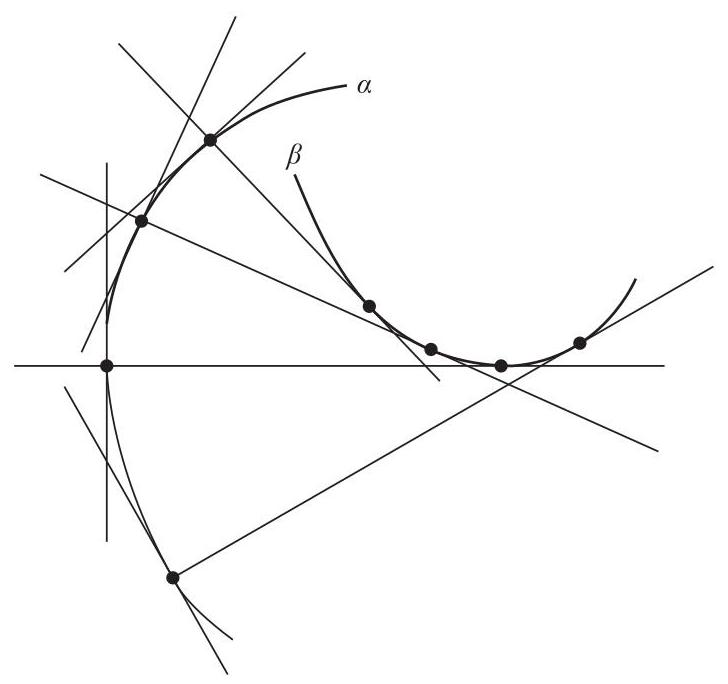
\includegraphics[max width=0.6\textwidth]{images/bo_d4b9jf3ef24c73e0334g_36_420_189_728_684_0.jpg}
\end{center}
\hspace*{3em} 

图 1-17

8. 参数化曲线(任意参数)的轨迹

\[
\alpha \left( t\right)  = \left( {t,\cosh t}\right) ,\;t \in  R,
\]

称为悬链线.

a. 证明悬链线的符号曲率(参见备注 1)为

\[
k\left( t\right)  = \frac{1}{{\cosh }^{2}t}.
\]

b. 证明悬链线的渐屈线(参见练习 7)为

\[
\beta \left( t\right)  = \left( {t - \sinh t\cosh t,2\cosh t}\right) .
\]

9. 给定一个可微函数 \(k\left( s\right) ,s \in  I\) ，证明具有 \(k\left( s\right)  = k\) 作为曲率的参数化平面曲线由下式给出

\[
\alpha \left( s\right)  = \left( {\int \cos \theta \left( s\right) {ds} + a,\int \sin \theta \left( s\right) {ds} + b}\right) ,
\]

其中

\[
\theta \left( s\right)  = \int k\left( s\right) {ds} + \varphi ,
\]

且曲线由向量 \(\left( {a,b}\right)\) 的平移和角度 \(\varphi\) 的旋转确定.

10. 考虑映射

\[
\alpha \left( t\right)  = \left\{  \begin{array}{ll} \left( {t,0,{e}^{-1/{t}^{2}}}\right) , & t > 0 \\  \left( {t,{e}^{-1/{t}^{2}},0}\right) , & t < 0 \\  \left( {0,0,0}\right) , & t = 0 \end{array}\right.
\]

a. 证明 \(\alpha\) 是一个可微曲线.

b. 证明对于所有 \(t\) ， \(\alpha\) 是正则的，并且曲率 \(k\left( t\right)  \neq  0\) ，对于 \(t \neq  0,t \neq   \pm  \sqrt{2/3}\) ，以及 \(k\left( 0\right)  = 0\) .

c. 表明当 \(t \rightarrow  0,t > 0\) 时，密切平面的极限是平面 \(y = 0\) ，但当 \(t \rightarrow  0,t < 0\) 时，密切平面的极限是平面 \(z = 0\) (这表明法向量在 \(t = 0\) 处不连续，并解释了为什么我们排除了 \(k = 0\) 的点).

d. 表明可以定义 \(\tau\) 以便 \(\tau  \equiv  0\) ，即使 \(\alpha\) 不是平面曲线.

11. 通常用极坐标表示平面曲线，由 \(\rho  = \rho \left( \theta \right)\) ， \(a \leq  \theta  \leq  b.\) 给出

a. 表明弧长是

\[
{\int }_{a}^{b}\sqrt{{\rho }^{2} + {\left( {\rho }^{\prime }\right) }^{2}}{d\theta }
\]

其中撇号表示相对于 \(\theta\) 的导数.

b. 表明曲率是

\[
k\left( \theta \right)  = \frac{2{\left( {\rho }^{\prime }\right) }^{2} - \rho {\rho }^{\prime \prime } + {\rho }^{2}}{{\left\{  {\left( {\rho }^{\prime }\right) }^{2} + {\rho }^{2}\right\}  }^{3/2}}.
\]

12. 令 \(\alpha  : I \rightarrow  {R}^{3}\) 为一条正则参数化曲线(不一定是弧长参数化)，令 \(\beta  : J \rightarrow  {R}^{3}\) 为 \(\alpha \left( I\right)\) 关于弧长 \(s = s\left( t\right)\) 的重参数化，从 \({t}_{0} \in  I\) 开始测量(见注 2).令 \(t = t\left( s\right)\) 为 \(s\) 的反函数，并设置 \({d\alpha }/{dt} = {\alpha }^{\prime },{d}^{2}\alpha /d{t}^{2} = {\alpha }^{\prime \prime }\) 等.证明

a. \({dt}/{ds} = 1/\left| {\alpha }^{\prime }\right| ,{d}^{2}t/d{s}^{2} =  - \left( {{\alpha }^{\prime } \cdot  {\alpha }^{\prime \prime }/{\left| {\alpha }^{\prime }\right| }^{4}}\right)\) .

b. \(\alpha\) 在 \(t \in  I\) 处的曲率是

\[
k\left( t\right)  = \frac{\left| {\alpha }^{\prime } \land  {\alpha }^{\prime \prime }\right| }{{\left| {\alpha }^{\prime }\right| }^{3}}.
\]

c. \(\alpha\) 在 \(t \in  I\) 处的挠率是

\[
\tau \left( t\right)  =  - \frac{\left( {{\alpha }^{\prime } \land  {\alpha }^{\prime \prime }}\right)  \cdot  {\alpha }^{\prime \prime \prime }}{{\left| {\alpha }^{\prime } \land  {\alpha }^{\prime \prime }\right| }^{2}}.
\]

d. 如果 \(\alpha  : I \rightarrow  {R}^{2}\) 是平面曲线 \(\alpha \left( t\right)  = \left( {x\left( t\right) ,y\left( t\right) }\right)\) ，则 \(\alpha\) 在 \(t\) 处的符号曲率(见注 1)是

\[
k\left( t\right)  = \frac{{x}^{\prime }{y}^{\prime \prime } - {x}^{\prime \prime }{y}^{\prime }}{{\left( {\left( {x}^{\prime }\right) }^{2} + {\left( {y}^{\prime }\right) }^{2}\right) }^{3/2}}.
\]

*13. 假设对于所有 \(s \in  I\) ， \(\tau \left( s\right)  \neq  0\) 和 \({k}^{\prime }\left( s\right)  \neq  0\) .证明 \(\alpha \left( I\right)\) 位于球体上的充要条件是

\[
{R}^{2} + {\left( {R}^{\prime }\right) }^{2}{T}^{2} = \text{ const., }
\]

其中 \(R = 1/k,T = 1/\tau\) ，以及 \({R}^{\prime }\) 是 \(R\) 相对于 \(s\) 的导数.

14. 设 \(\alpha  : \left( {a,b}\right)  \rightarrow  {R}^{2}\) 为一条正则参数化平面曲线.假设存在 \({t}_{0},a < {t}_{0} < b\) ，使得原点到 \(\alpha\) 的轨迹的距离 \(\left| {\alpha \left( t\right) }\right|\) 在 \({t}_{0}\) 处取得最大值.证明 \(\alpha\) 在 \({t}_{0}\) 处的曲率 \(k\) 满足 \(\left| {k\left( {t}_{0}\right) }\right|  \geq  1/\left| {\alpha \left( {t}_{0}\right) }\right|\) .

*15. 表明，已知一条具有处处非零挠率的曲线 \(\alpha\) 的向量函数 \(b = b\left( s\right)\) (副法线向量)，可以确定该曲线的曲率 \(k\left( s\right)\) 和挠率的绝对值 \(\tau \left( s\right)\) .

*16. 表明，已知一条具有处处非零挠率的曲线 \(\alpha\) 的向量函数 \(n = n\left( s\right)\) (法线向量)，可以确定该曲线的曲率 \(k\left( s\right)\) 和挠率 \(\tau \left( s\right)\) .

17. 一般而言，如果曲线 \(\alpha\) 的切线与某个固定方向成恒定角度，则称该曲线为螺旋线.假设 \(\tau \left( s\right)  \neq  0,s \in  I\) ，并证明:

*a. \(\alpha\) 是螺旋线当且仅当 \(k/\tau  =\) 为常数.

*b. \(\alpha\) 是螺旋线当且仅当包含 \(n\left( s\right)\) 并通过 \(\alpha \left( s\right)\) 的直线平行于某个固定平面.

*c. \(\alpha\) 是螺旋线当且仅当包含 \(b\left( s\right)\) 并通过 \(\alpha \left( s\right)\) 的直线与某个固定方向成恒定角度.

d. 曲线

\[
\alpha \left( s\right)  = \left( {\frac{a}{c}\int \sin \theta \left( s\right) {ds},\frac{a}{c}\int \cos \theta \left( s\right) {ds},\frac{b}{c}s}\right) ,
\]

其中 \({c}^{2} = {a}^{2} + {b}^{2}\) 是螺旋线，并且 \(k/\tau  = a/b\) .

*18. 设 \(\alpha  : I \rightarrow  {R}^{3}\) 为一条参数化的正则曲线(不一定是弧长参数化)，且满足 \(k\left( t\right)  \neq  0,\tau \left( t\right)  \neq  0,t \in  I\) .如果存在一条曲线 \(\overline{\alpha } : I \rightarrow  {R}^{3}\) ，使得 \(\alpha\) 和 \(\overline{\alpha }\) 在 \(t \in  I\) 处的法线相同，则称曲线 \(\alpha\) 为一条 Bertrand 曲线.在这种情况下， \(\overline{\alpha }\) 被称为 \(\alpha\) 的 Bertrand 伴侣，我们可以写成

\[
\overline{\alpha }\left( t\right)  = \alpha \left( t\right)  + {rn}\left( t\right) .
\]

证明

a. \(r\) 是常数.

b. \(\alpha\) 是 Bertrand 曲线当且仅当存在一个线性关系

\[
{Ak}\left( t\right)  + {B\tau }\left( t\right)  = 1,\;t \in  I,
\]

其中 \(A,B\) 是非零常数，而 \(k\) 和 \(\tau\) 分别是 \(\alpha\) 的曲率和挠率.

c. 如果 \(\alpha\) 有不止一个 Bertrand 伴侣，则它有无穷多个 Bertrand 伴侣.这种情况当且仅当 \(\alpha\) 是一个圆螺旋线.

\section{局部正则形式\footnote{本节可在初读时省略.}}

解决几何问题最有效的方法之一是找到一个适合该问题的坐标系.在研究曲线局部性质时，在点 \(s\) 的邻域内，我们有一个自然的坐标系，即点 \(s\) 处的Frenet三脚架.因此，将曲线参照这个三脚架来描述是方便的.

设 \(\alpha  : I \rightarrow  {R}^{3}\) 为一条由弧长参数化的、没有一阶奇异点的曲线.我们将使用 \(t\left( {s}_{0}\right) ,n\left( {s}_{0}\right) ,b\left( {s}_{0}\right)\) 三脚架作为 \({R}^{3}\) 的基底，在 \({s}_{0}\) 的邻域内写出该曲线的方程.我们可以无损地假设 \({s}_{0} = 0\) ，并且我们将考虑(有限的)泰勒展开式

\[
\alpha \left( s\right)  = \alpha \left( 0\right)  + s{\alpha }^{\prime }\left( 0\right)  + \frac{{s}^{2}}{2}{\alpha }^{\prime \prime }\left( 0\right)  + \frac{{s}^{3}}{6}{\alpha }^{\prime \prime \prime }\left( 0\right)  + R,
\]

其中 \(\mathop{\lim }\limits_{{s \rightarrow  0}}R/{s}^{3} = 0\) .因为 \({\alpha }^{\prime }\left( 0\right)  = t,{\alpha }^{\prime \prime }\left( 0\right)  = {kn}\) ，并且

\[
{\alpha }^{\prime \prime \prime }\left( 0\right)  = {\left( kn\right) }^{\prime } = {k}^{\prime }n + k{n}^{\prime } = {k}^{\prime }n - {k}^{2}t - {k\tau b},
\]

我们得到

\[
\alpha \left( s\right)  - \alpha \left( 0\right)  = \left( {s - \frac{{k}^{2}{s}^{3}}{3!}}\right) t + \left( {\frac{{s}^{2}k}{2} + \frac{{s}^{3}{k}^{\prime }}{3!}}\right) n - \frac{{s}^{3}}{3!}{k\tau b} + R,
\]

其中所有项都在 \(s = 0\) 处计算.

现在我们取 Oxyz 系统，使得原点 \(O\) 与 \(\alpha \left( 0\right)\) 重合，并且 \(t = \left( {1,0,0}\right) ,n = \left( {0,1,0}\right) ,b = \left( {0,0,1}\right)\) .在这些条件下， \(\alpha \left( s\right)  = \left( {x\left( s\right) ,y\left( s\right) ,z\left( s\right) }\right)\) 由下式给出

\[
x\left( s\right)  = s - \frac{{k}^{2}{s}^{3}}{6} + {R}_{x},
\]

\[
y\left( s\right)  = \frac{k}{2}{s}^{2} + \frac{{k}^{\prime }{s}^{3}}{6} + {R}_{y}, \tag{1}
\]

\[
z\left( s\right)  =  - \frac{k\tau }{6}{s}^{3} + {R}_{z}
\]



其中 \(R = \left( {{R}_{x},{R}_{y},{R}_{z}}\right)\) .表达式 (1) 被称为 \(\alpha\) 在 \(s = 0\) 邻域内的局部正则形式.图 1-18 是 \(\alpha\) 的轨迹在 \(s\) 很小时在 \({tn},{tb}\) 和 \({nb}\) 平面上的投影的粗略草图.

\begin{center}
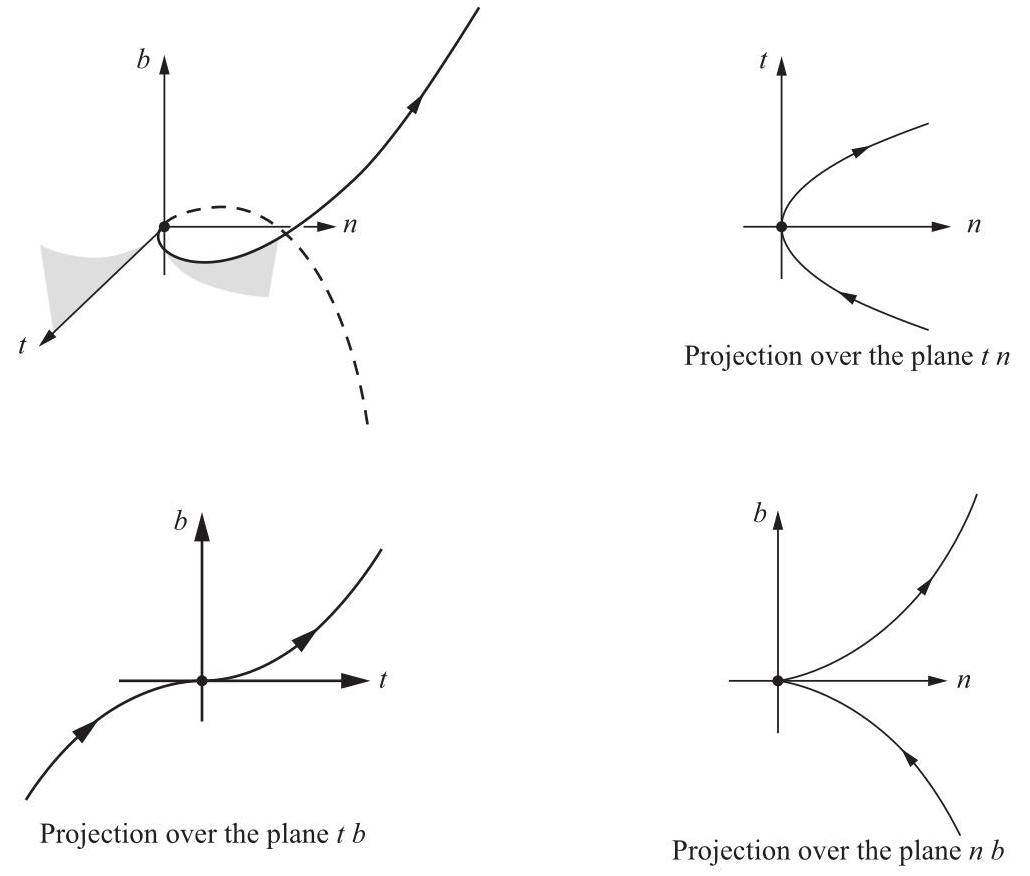
\includegraphics[max width=0.9\textwidth]{images/bo_d4b9jf3ef24c73e0334g_40_270_697_1030_876_0.jpg}
\end{center}
\hspace*{3em} 

图 1-18

下面我们将描述局部正则形式的一些几何应用.在练习题中会找到更多应用.

第一个应用是对挠率符号的以下解释.从 (1) 的第三个方程可知，如果 \(\tau  < 0\) 且 \(s\) 足够小，则 \(z\left( s\right)\) 随 \(s\) 增大而增大.我们约定将密切平面(osculating plane)的“正侧”定义为 \(b\) 指向的一侧.那么，由于 \(z\left( 0\right)  = 0\) ，当我们沿着弧长增大的方向描述曲线时，曲线将在 \(s = 0\) 处穿过密切平面，指向正侧(见图 1-19).反之，如果 \(\tau  > 0\) ，则曲线(沿着弧长增大的方向描述)将穿过密切平面，指向与正侧相反的一侧.

\begin{center}
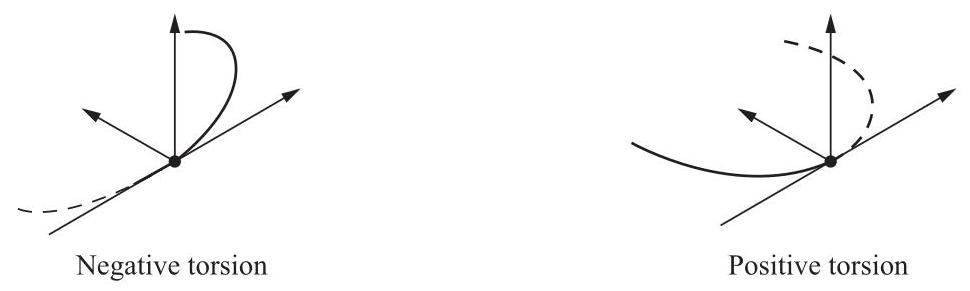
\includegraphics[max width=0.8\textwidth]{images/bo_d4b9jf3ef24c73e0334g_41_279_387_970_291_0.jpg}
\end{center}
\hspace*{3em} 

图 1-19

第 1-5 节练习 1 中的螺旋线具有负挠率.具有正挠率的曲线的一个例子是螺旋线

\[
\alpha \left( s\right)  = \left( {a\cos \frac{s}{c},a\sin \frac{s}{c}, - b\frac{s}{c}}\right)
\]

通过在 \({xz}\) 平面上进行反射从第一条螺旋线得到(见图 1-19).

注.通常也通过 \({b}^{\prime } =  - {\tau n}\) 来定义挠率.使用这种定义，练习 1 中螺旋线的挠率将变为正值.

标准形式的另一个结果是，存在 \(J \subset  I\) 的一个邻域 \(s = 0\) ，使得 \(\alpha \left( J\right)\) 完全包含在化直平面朝向向量 \(n\) 所指方向的一侧(见图 1 - 18).事实上，由于 \(k > 0\) ，对于足够小的 \(s\) ，我们有 \(y\left( s\right)  \geq  0\) ，并且当且仅当 \(s = 0\) 时，有 \(y\left( s\right)  = 0\) .这就证明了我们的断言.

作为正则形式的最后一个应用，我们提到密切平面具有以下性质.密切平面在 \(s\) 处是切线在 \(s\) 处确定的平面与点 \(\alpha \left( {s + h}\right)\) 所确定的平面当 \(h \rightarrow  0\) 时的极限位置.为了证明这一点，我们假设 \(s = 0\) .因此，包含在 \(s = 0\) 处的切线的任何平面都具有 \(z = {cy}\) 或 \(y = 0\) 的形式.平面 \(y = 0\) 是切面，如上所述，它不包含 \(\alpha \left( 0\right)\) 附近的任何点(除了 \(\alpha \left( 0\right)\) 本身)，因此可以从我们的考虑中排除.平面 \(z = {cy}\) 通过 \(\alpha \left( {s + h}\right)\) 的条件是 \(\left( {s = 0}\right)\) .

\[
c = \frac{z\left( h\right) }{y\left( h\right) } = \frac{-\frac{k}{6}\tau {h}^{3} + \cdots }{\frac{k}{2}{h}^{2} + \frac{{k}^{2}}{6}{h}^{3} + \cdots }.
\]

令 \(h \rightarrow  0\) ，我们看到 \(c \rightarrow  0\) .因此，平面 \(z\left( s\right)  = c\left( h\right) y\left( s\right)\) 的极限位置是平面 \(z = 0\) ，即密切平面，正如我们所希望的.

\exerciseline

*1. 令 \(\alpha  : I \rightarrow  {R}^{3}\) 为由弧长参数化的曲线，其曲率为 \(k\left( s\right)  \neq  0,s \in  I\) .令 \(P\) 为满足以下两个条件的平面:

1. \(P\) 包含 \(s\) 处的切线.

2. 对于 \(s\) 的任何邻域 \(J \subset  I\) ，在 \(P\) 的两侧都存在 \(\alpha \left( J\right)\) 的点.

证明 \(P\) 是 \(\alpha\) 在 \(s\) 处的密切平面.

2. 令 \(\alpha  : I \rightarrow  {R}^{3}\) 为由弧长参数化的曲线，其曲率为 \(k\left( s\right)  \neq  0,s \in  I\) .证明

*a. 密切平面在 \(s\) 处是经过 \(\alpha \left( s\right) ,\alpha \left( {s + {h}_{1}}\right) ,\alpha \left( {s + {h}_{2}}\right)\) 的平面当 \({h}_{1},{h}_{2} \rightarrow  0\) 时的极限位置.

b. 经过 \(\alpha \left( s\right) ,\alpha \left( {s + {h}_{1}}\right)\) 、 \(\alpha \left( {s + {h}_{2}}\right)\) 的圆当 \({h}_{1},{h}_{2} \rightarrow  0\) 时的极限位置是密切平面 \(s\) 中的一个圆，其圆心在包含 \(n\left( s\right)\) 的直线上，其半径为曲率半径 \(1/k\left( s\right)\) ；这个圆称为密切圆，在 \(s\) 处.

3. 证明正则参数化曲线 \(\alpha  : I \rightarrow \; {R}^{3}\) 的曲率 \(k\left( t\right)  \neq  0\) 等于平面曲线 \(\pi  \circ  \alpha\) 在 \(t\) 处的曲率，其中 \(\pi\) 是 \(\alpha\) 在 \(t\) 处密切平面上的法向投影.

\section{平面曲线的全局性质\footnote{本节在初读时可以省略.}}

在本节中，我们希望描述一些属于曲线全局微分几何的结果.即使在平面曲线的简单情况下，该主题也已经提供了非平凡定理和有趣问题的例子.为了在此处发展这些材料，我们必须假设一些合理的、无需证明的事实；我们将尽量通过精确陈述这些事实来做到这一点.尽管我们希望稍后以更系统的方式回到全局微分几何(第 5 章)，但我们相信早期介绍该主题既能激发兴趣，又能起到指导作用.

本节包含三个主题，难度递增:(A) 等周不等式，(B) 四顶点定理，以及 (C) Cauchy-Crofton 公式.这些主题完全独立，在初读时可以省略其中一些或全部.

闭区间 \(\left\lbrack  {a,b}\right\rbrack\) 上的可微函数是包含 \(\left\lbrack  {a,b}\right\rbrack\) 的开区间上定义的可微函数的限制.




闭合平面曲线是指一个正则参数化曲线 \(\alpha  : \left\lbrack  {a,b}\right\rbrack   \rightarrow  {R}^{2}\) ，使得 \(\alpha\) 成立，并且其所有导数在 \(a\) 和 \(b\) 处相等；也就是说，

\[
\alpha \left( a\right)  = \alpha \left( b\right) ,\;{\alpha }^{\prime }\left( a\right)  = {\alpha }^{\prime }\left( b\right) ,\;{\alpha }^{\prime \prime }\left( a\right)  = {\alpha }^{\prime \prime }\left( b\right) ,\ldots .
\]

曲线 \(\alpha\) 是简单的，如果它没有进一步的自交点；也就是说，如果 \({t}_{1},{t}_{2} \in \; \lbrack a,b),{t}_{1} \neq  {t}_{2}\) ，那么 \(\alpha \left( {t}_{1}\right)  \neq  \alpha \left( {t}_{2}\right)\) (图 1-20).

\begin{center}
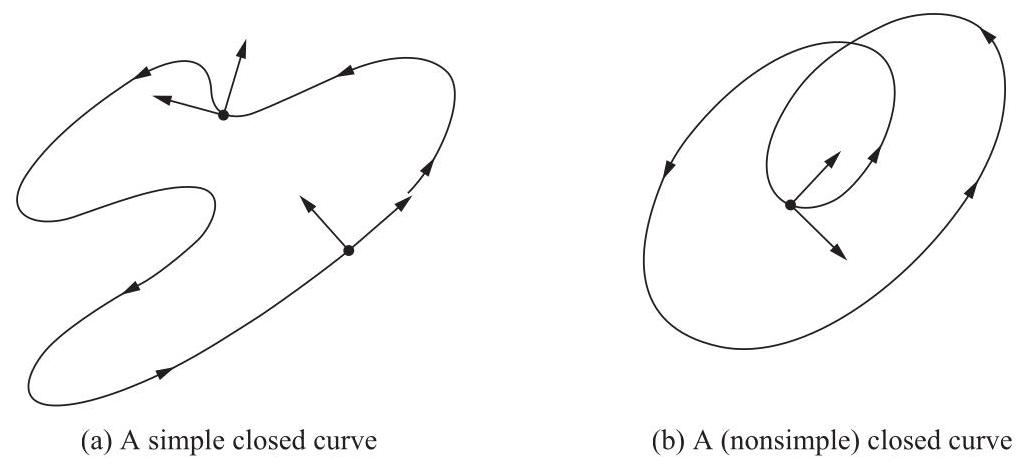
\includegraphics[max width=0.9\textwidth]{images/bo_d4b9jf3ef24c73e0334g_43_255_543_1026_470_0.jpg}
\end{center}
\hspace*{3em} 

图 1-20

\begin{center}
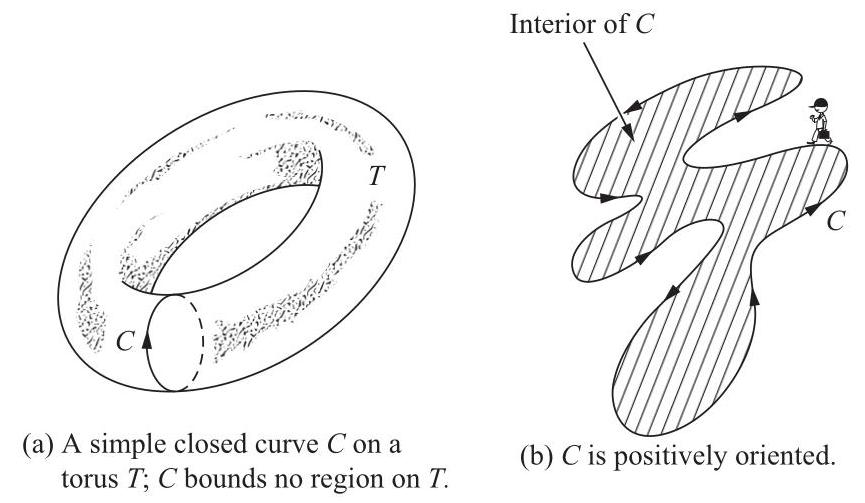
\includegraphics[max width=0.7\textwidth]{images/bo_d4b9jf3ef24c73e0334g_43_334_1143_865_503_0.jpg}
\captionof{figure}{}
\end{center}

我们通常考虑由弧长 \(s\) 参数化的曲线 \(\alpha  : \left\lbrack  {0,l}\right\rbrack   \rightarrow  {R}^{2}\) ；因此， \(l\) 是 \(\alpha\) 的长度.有时我们称一个简单的闭合曲线 \(C\) ，意指这样一个对象的轨迹.曲线 \(\alpha\) 的曲率将带有符号，如第 1-5 节的注记 1 中所示 (见图 1-20).

我们假设平面上的一个简单闭合曲线 \(C\) 围成该平面的一块区域，称为 \(C\) 的内部.这是所谓的若尔当曲线定理的一部分 (证明将在第 5-7 节，定理 1 中给出)，该定理例如不适用于环面上的简单曲线 (甜甜圈的表面；见图 1-21(a)).每当我们谈论由简单闭合曲线 \(C\) 围成的面积时，我们指的是 \(C\) 内部的面积.我们进一步假设，简单闭合曲线的参数可以选择得使得，当沿着曲线以参数增大的方向前进时，曲线的内部保持在左侧 (图 l-21(b)).这样的曲线将被称为正定向的.

\subsection*{A. 等周不等式}

这也许是微分几何中最古老的全局定理，并且与以下 (等周) 问题有关.在具有给定长度 \(l\) 的所有平面上的简单闭合曲线中，哪一条围成的面积最大？以这种形式，这个问题是古希腊人已知的，他们也知道答案，即圆.然而，对圆是等周问题解这一事实的令人满意的证明花了很长时间才出现.主要原因似乎是早期证明假设解应该存在.直到 1870 年，K. Weierstrass 指出许多类似的问题没有解，并给出了等周问题解存在性的完整证明.Weierstrass 的证明有些困难，因为它是一个他为处理最大化 (或最小化) 特定积分的问题而开发的理论的推论 (该理论称为变分学，等周问题是它处理的问题的一个典型例子).后来，人们找到了更直接的证明.我们将要介绍的简单证明是 E. Schmidt (1939) 的成果.对于另一个直接证明和该主题的进一步参考文献，可以参考参考文献 [10].

我们将使用以下公式计算由正定向的简单闭合曲线 \(\alpha \left( t\right)  = \left( {x\left( t\right) ,y\left( t\right) }\right)\) 围成的面积 \(A\) ，其中 \(t \in  \left\lbrack  {a,b}\right\rbrack\) 是任意参数:

\[
A =  - {\int }_{a}^{b}y\left( t\right) {x}^{\prime }\left( t\right) {dt} = {\int }_{a}^{b}x\left( t\right) {y}^{\prime }\left( t\right) {dt} = \frac{1}{2}{\int }_{a}^{b}\left( {x{y}^{\prime } - y{x}^{\prime }}\right) {dt} \tag{1}
\]

请注意，第二个公式是通过观察以下事实从第一个公式得到的:

\[
{\int }_{a}^{b}x{y}^{\prime }{dt} = {\int }_{a}^{b}{\left( xy\right) }^{\prime }{dt} - {\int }_{a}^{b}{x}^{\prime }{ydt} = \left\lbrack  {{xy}\left( b\right)  - {xy}\left( a\right) }\right\rbrack   - {\int }_{a}^{b}{x}^{\prime }{ydt}
\]

\[
=  - {\int }_{a}^{b}{x}^{\prime }{ydt}
\]

因为曲线是闭合的.第三个公式可以从前两个公式直接得到.

为了证明公式 (1) 中的第一个公式，我们最初考虑图 1-22 的情况，其中曲线由两条平行于 \(y\) 轴的直线段和两条可以写成以下形式的弧组成:

\[
y = {f}_{1}\left( x\right) \text{ and }y = {f}_{2}\left( x\right) ,x \in  \left\lbrack  {{x}_{0},{x}_{1}}\right\rbrack  ,{f}_{1} > {f}_{2}.
\]

\begin{center}
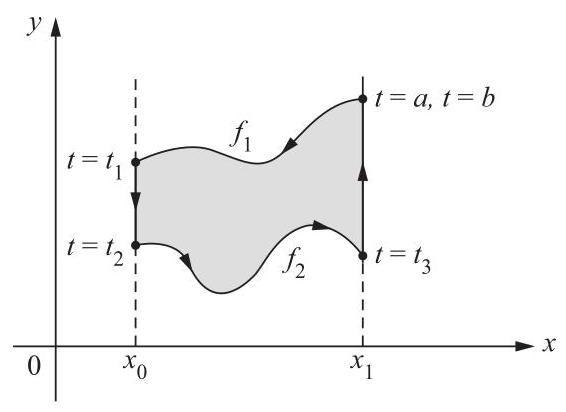
\includegraphics[max width=0.5\textwidth]{images/bo_d4b9jf3ef24c73e0334g_45_179_199_566_412_0.jpg}
\captionof{figure}{}
\end{center}

显然，曲线围成的面积是

\[
A = {\int }_{{x}_{0}}^{{x}_{1}}{f}_{1}\left( x\right) {dx} - {\int }_{{x}_{0}}^{{x}_{1}}{f}_{2}\left( x\right) {dx}.
\]

由于曲线是正定向的，根据图 1-22 的符号，我们得到:

\[
A =  - {\int }_{a}^{{t}_{1}}y\left( t\right) {x}^{\prime }\left( t\right) {dt} - {\int }_{{t}_{2}}^{{t}_{3}}y\left( t\right) {x}^{\prime }\left( t\right) {dt} =  - {\int }_{a}^{b}y\left( t\right) {x}^{\prime }\left( t\right) {dt},
\]

因为 \({x}^{\prime }\left( t\right)  = 0\) 沿着平行于 \(y\) 轴的线段.这证明了这种情况下的公式 (1).

为了证明一般情况，必须证明可以将由曲线所围成的区域划分为有限个上述类型的区域.这显然是可能的(图 1-23)，如果平面中存在一条直线 \(E\) ，使得 \(\alpha \left( t\right)\) 到这条直线的距离 \(\rho \left( t\right)\) 是一个只有有限个临界点的函数(临界点是 \({\rho }^{\prime }\left( t\right)  = 0\) 的点).最后一个论断是正确的，但我们不深入证明.我们在此提及，方程 (1) 也可以通过使用平面上的斯托克斯(格林)定理得到(参见练习 15).

定理 1(等周不等式).设 \(\mathrm{C}\) 为一条长度为 \(l\) 的简单闭合平面曲线，设 \(\mathrm{A}\) 为 \(\mathrm{C}\) 所围成区域的面积.则

\[
{l}^{2} - {4\pi }\mathrm{A} \geq  0, \tag{2}
\]

当且仅当 \(\mathrm{C}\) 是一个圆时，等号成立.

证明.设 \(E\) 和 \({E}^{\prime }\) 是两条不与闭合曲线 \(C\) 相交的平行直线，并将它们一起移动，直到它们首次与 \(C\) 相交.我们 thus 得到两条平行切线 \(C,L\) 和 \({L}^{\prime }\) ，因此曲线完全包含在 \(L\) 和 \({L}^{\prime }\) 所围成的带状区域内.考虑一个圆 \({S}^{1}\) ，它与 \(L\) 和 \({L}^{\prime }\) 都相切，并且不与 \(C\) 相交.设 \(O\) 为 \({S}^{1}\) 的圆心，并取一个以 \(O\) 为原点且 \(x\) 轴垂直于 \(L\) 和 \({L}^{\prime }\) 的坐标系(图 1-24).用弧长 \(\alpha \left( s\right)  = \left( {x\left( s\right) ,y\left( s\right) }\right)\) 参数化 \(C\) ，使其定向为正，并且 \(L\) 和 \({L}^{\prime }\) 的切点分别为 \(s = 0\) 和 \(s = {s}_{1}\) .

\begin{center}
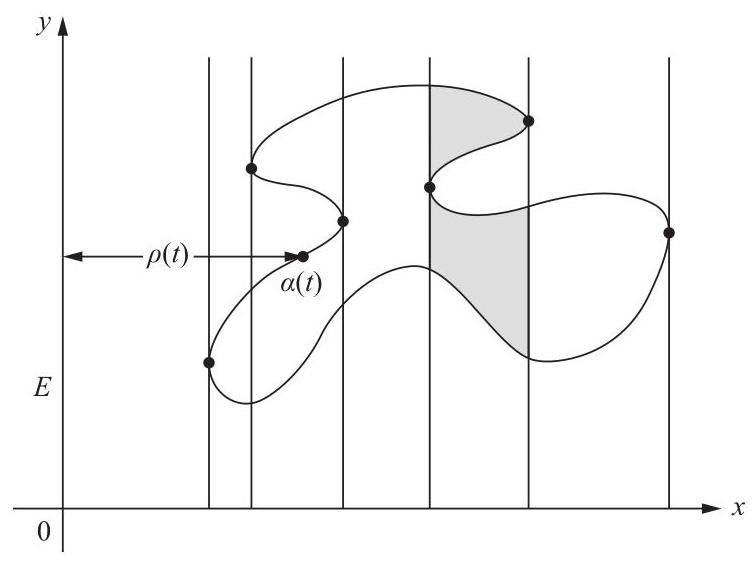
\includegraphics[max width=0.6\textwidth]{images/bo_d4b9jf3ef24c73e0334g_46_405_564_756_561_0.jpg}
\captionof{figure}{}
\end{center}

\begin{center}
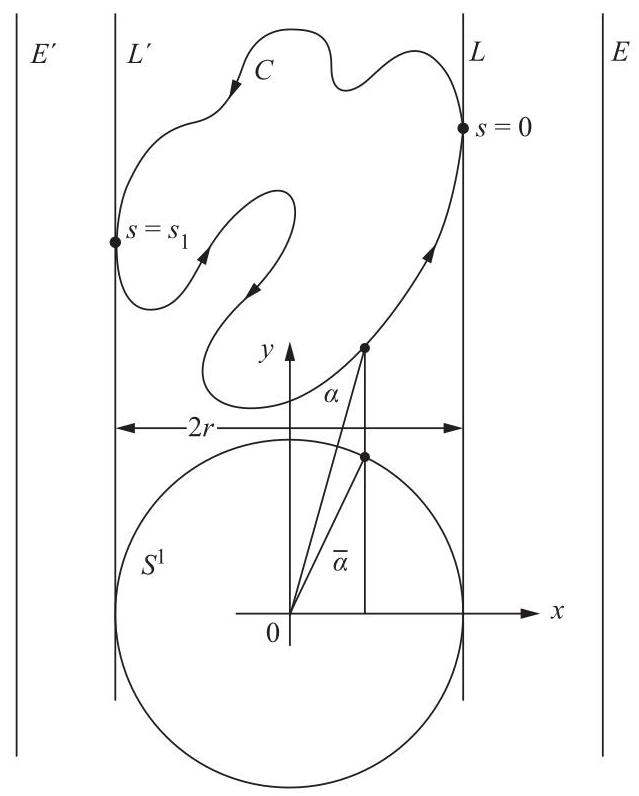
\includegraphics[max width=0.5\textwidth]{images/bo_d4b9jf3ef24c73e0334g_46_460_1245_639_796_0.jpg}
\captionof{figure}{}
\end{center}

我们可以假设 \({S}^{1}\) 的方程是

\[
\overline{\alpha }\left( s\right)  = \left( {\bar{x}\left( s\right) ,\bar{y}\left( s\right) }\right)  = \left( {x\left( s\right) ,\bar{y}\left( s\right) }\right) ,s \in  \left\lbrack  {0,l}\right\rbrack  .
\]

设 \({2r}\) 为 \(L\) 和 \({L}^{\prime }\) 之间的距离.通过使用方程 (1) 并用 \(\bar{A}\) 表示 \({S}^{1}\) 所围成的面积，我们得到

\[
A = {\int }_{0}^{l}x{y}^{\prime }{ds},\;\bar{A} = \pi {r}^{2} =  - {\int }_{0}^{l}\bar{y}{x}^{\prime }{ds}.
\]

因此，

\[
A + \pi {r}^{2} = {\int }_{0}^{l}\left( {x{y}^{\prime } - \bar{y}{x}^{\prime }}\right) {ds} \leq  {\int }_{0}^{l}\sqrt{{\left( x{y}^{\prime } - \bar{y}{x}^{\prime }\right) }^{2}}{ds}
\]

\[
\leq  {\int }_{0}^{l}\sqrt{\left( {{x}^{2} + {\bar{y}}^{2}}\right) \left( {{\left( {x}^{\prime }\right) }^{2} + {\left( {y}^{\prime }\right) }^{2}}\right) }{ds} = {\int }_{0}^{l}\sqrt{{\bar{x}}^{2} + {\bar{y}}^{2}}{ds} \tag{3}
\]

\[
= {lr}\text{ , }
\]

其中我们使用了两个向量 \({v}_{1}\) 和 \({v}_{2}\) 的内积满足

\[
{\left| \left( {v}_{1} \cdot  {v}_{2}\right) \right| }^{2} \leq  {\left| \left( {v}_{1}\right) \right| }^{2}{\left| \left( {v}_{2}\right) \right| }^{2}.
\]
 (3')

在证明的后续部分，我们将需要等号在 (3') 中成立当且仅当一个向量是另一个向量的倍数.

我们现在注意到两个正数的几何平均小于或等于它们的算术平均，并且当且仅当它们相等时，等号成立.由此得出

\[
\sqrt{A}\sqrt{\pi {r}^{2}} \leq  \frac{1}{2}\left( {A + \pi {r}^{2}}\right)  \leq  \frac{1}{2}{lr}. \tag{4}
\]

因此， \({4\pi A}{r}^{2} \leq  {l}^{2}{r}^{2}\) ，这就得到了方程 (2).

现在，假设方程 (2) 中的等号成立.那么等号必须在方程 (3) 和 (4) 的所有地方都成立.从方程 (4) 中的等号可以得出 \(A = \pi {r}^{2}\) .因此， \(l = {2\pi r}\) 和 \(r\) 不依赖于 \(L\) 方向的选择.此外，方程 (3) 中的等号意味着

\[
\left( {x,\bar{y}}\right)  = \lambda \left( {{y}^{\prime }, - {x}^{\prime }}\right)
\]

即，

\[
\lambda  = \frac{x}{{y}^{\prime }} = \frac{\bar{y}}{{x}^{\prime }} = \frac{\sqrt{{x}^{2} + {\bar{y}}^{2}}}{\sqrt{{\left( {y}^{\prime }\right) }^{2} + {\left( {x}^{\prime }\right) }^{2}}} =  \pm  r.
\]

因此， \(x =  \pm  r{y}^{\prime }\) .由于 \(r\) 不依赖于 \(L\) 方向的选择，我们可以将 \(x\) 和 \(y\) 在最后一个关系式中互换，得到 \(y =  \pm  r{x}^{\prime }\) .因此，

\[
{x}^{2} + {y}^{2} = {r}^{2}\left( {{\left( {x}^{\prime }\right) }^{2} + {\left( {y}^{\prime }\right) }^{2}}\right)  = {r}^{2}
\]

和 \(C\) 是一个圆，正如我们所愿.Q.E.D.

注1. 很容易验证上述证明可以应用于 \({C}^{1}\) 曲线，即曲线 \(\alpha \left( t\right)  = \left( {x\left( t\right) ,y\left( t\right) }\right) ,t \in  \left\lbrack  {a,b}\right\rbrack\) ，对于这类曲线，我们只要求函数 \(x\left( t\right) ,y\left( t\right)\) 具有连续的一阶导数(当然，如果曲线是闭合的，这些导数在 \(a\) 和 \(b\) 处是相等的).

注2. 等周不等式对于一大类曲线都成立.直接证明表明，只要我们能定义所考虑曲线的弧长和面积，证明就有效.为了便于应用，需要指出该定理对于分段 \({C}^{1}\) 曲线成立，即由有限个 \({C}^{1}\) 弧组成的连续曲线.这些曲线可以有有限个角点，切线在此处不连续(图1-25).

\begin{center}
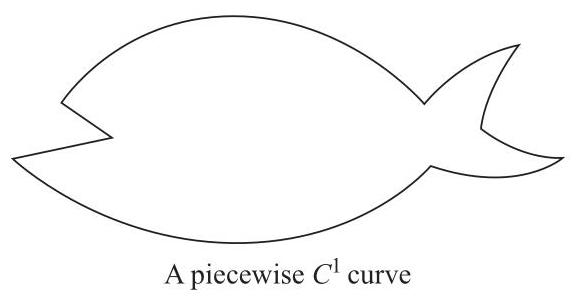
\includegraphics[max width=0.5\textwidth]{images/bo_d4b9jf3ef24c73e0334g_48_198_926_576_296_0.jpg}
\captionof{figure}{图1-25}
\end{center}

\subsection*{B. 四顶点定理}

我们将需要关于平面闭合曲线的进一步一般事实.

设 \(\alpha  : \left\lbrack  {0,l}\right\rbrack   \rightarrow  {R}^{2}\) 是由 \(\alpha \left( s\right)  = \left( {x\left( s\right) ,y\left( s\right) }\right)\) 给出的平面闭合曲线.由于 \(s\) 是弧长，切向量 \(t\left( s\right)  = \left( {{x}^{\prime }\left( s\right) ,{y}^{\prime }\left( s\right) }\right)\) 的长度为单位长度.引入切线指示图 \(t : \left\lbrack  {0,l}\right\rbrack   \rightarrow  {R}^{2}\) 是方便的，它由 \(t\left( s\right)  = \left( {{x}^{\prime }\left( s\right) ,{y}^{\prime }\left( s\right) }\right)\) 给出；这是一个可微曲线，其轨迹包含在一个半径为1的圆内(图1-26).注意切线指示图的速度向量是

\[
\frac{dt}{ds} = \left( {{x}^{\prime \prime }\left( s\right) ,{y}^{\prime \prime }\left( s\right) }\right)
\]

\[
= {\alpha }^{\prime \prime }\left( s\right)  = {kn},
\]

其中 \(n\) 是法向量，方向与第1-5节注2中的相同， \(k\) 是 \(\alpha\) 的曲率.

\begin{center}
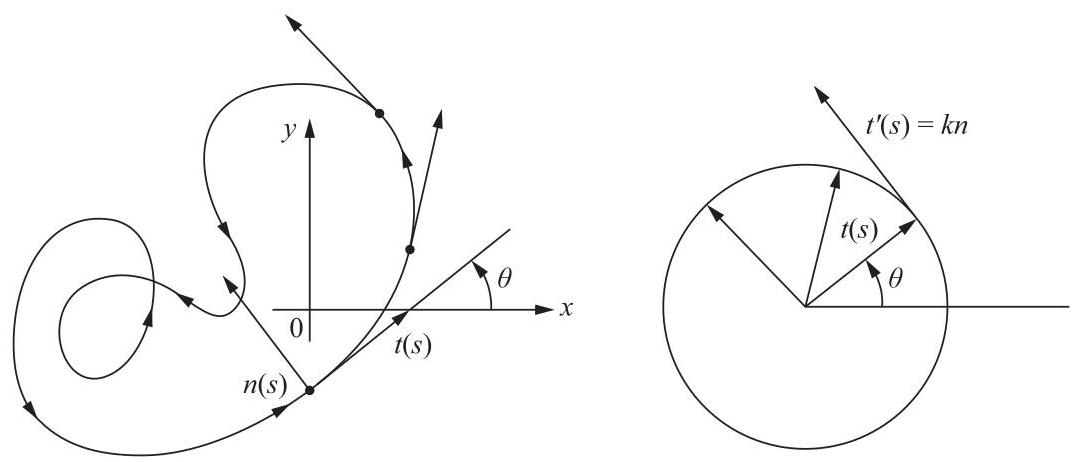
\includegraphics[max width=0.9\textwidth]{images/bo_d4b9jf3ef24c73e0334g_49_226_191_1084_462_0.jpg}
\captionof{figure}{图1-26}
\end{center}

设 \(\theta \left( s\right) ,0 < \theta \left( s\right)  < {2\pi }\) 是 \(t\left( s\right)\) 与 \(x\) 轴所成的角度；即 \({x}^{\prime }\left( s\right)  = \cos \theta \left( s\right) ,{y}^{\prime }\left( s\right)  = \sin \theta \left( s\right)\) .由于

\[
\theta \left( s\right)  = \arctan \frac{{y}^{\prime }\left( s\right) }{{x}^{\prime }\left( s\right) },
\]

\(\theta  = \theta \left( s\right)\) 在局部是良定义的(即，在每个 \(s\) 的小区间内是良定义的)作为一个可微函数，并且

\[
\frac{dt}{ds} = \frac{d}{ds}\left( {\cos \theta ,\sin \theta }\right)
\]

\[
= {\theta }^{\prime }\left( {-\sin \theta ,\cos \theta }\right)  = {\theta }^{\prime }n.
\]

这意味着 \({\theta }^{\prime }\left( s\right)  = k\left( s\right)\) ，并建议通过以下方式定义一个全局可微函数 \(\theta  : \left\lbrack  {0,l}\right\rbrack   \rightarrow  R\) :

\[
\theta \left( s\right)  = {\int }_{0}^{s}k\left( s\right) {ds}.
\]

由于

\[
{\theta }^{\prime } = k = {x}^{\prime }{y}^{\prime \prime } - {x}^{\prime \prime }{y}^{\prime } = {\left( \arctan \frac{{y}^{\prime }}{{x}^{\prime }}\right) }^{\prime },
\]

这个全局函数与前面局部定义的 \(\theta\) 在常数意义下是一致的.直观地说， \(\theta \left( s\right)\) 测量切向量的总旋转，即当我们将曲线 \(\alpha\) 从0跑到 \(s\) 时，切线指示图上点 \(t\left( s\right)\) 所描述的总角度.由于 \(\alpha\) 是闭合的，这个角度是 \({2\pi }\) 的整数倍 \(I\) ；即，

\[
{\int }_{o}^{l}k\left( s\right) {ds} = \theta \left( l\right)  - \theta \left( 0\right)  = {2\pi I}.
\]

整数 \(I\) 称为曲线 \(\alpha\) 的旋转指数.

图 1-27 展示了一些曲线及其转动指数的例子.请注意，当我们改变曲线的方向时，转动指数的符号会改变.此外，定义设置如下，使得正向简单闭合曲线的转动指数为正.

转动指数的一个重要全局事实包含在以下定理中，该定理将在本书后面(第 5-7 节，定理 2)证明.

转动切线定理.简单闭合曲线的转动指数为 \(\pm  1\) ，其符号取决于曲线的方向.

正则平面(不一定是闭合的)曲线 \(\alpha  : \left\lbrack  {a,b}\right\rbrack   \rightarrow  {R}^{2}\) 是凸的，如果对于所有 \(t \in  \left\lbrack  {a,b}\right\rbrack\) ， \(\alpha\) 的轨迹 \(\alpha \left( \left\lbrack  {a,b}\right\rbrack  \right)\) 完全位于由 \(t\) 处的切线确定的闭半平面的一侧(图 1-28).

正则平面曲线 \(\alpha  : \left\lbrack  {a,b}\right\rbrack   \rightarrow  {R}^{2}\) 的顶点是点 \(t \in  \left\lbrack  {a,b}\right\rbrack\) ，其中 \({k}^{\prime }\left( t\right)  = 0\) .例如，长短轴不相等的椭圆恰好有四个顶点，即轴与椭圆相交的点(参见练习 3).一个有趣的全局事实是，这是所有闭合凸曲线的最小顶点数.

定理 2(四顶点定理).简单闭合凸曲线至少有四个顶点.

在开始证明之前，我们需要一个引理.

引理.设 \(\alpha  : \left\lbrack  {0,l}\right\rbrack   \rightarrow  {\mathbb{R}}^{2}\) 为由弧长参数化的平面闭合曲线，设 A、B 和 C 为任意实数.则

\[
{\int }_{0}^{l}\left( {\mathrm{{Ax}} + \mathrm{{By}} + \mathrm{C}}\right) \frac{\mathrm{{dk}}}{\mathrm{{ds}}}\mathrm{{ds}} = 0, \tag{5}
\]

其中函数 \(\mathrm{x} = \mathrm{x}\left( \mathrm{s}\right) ,\mathrm{y} = \mathrm{y}\left( \mathrm{s}\right)\) 由 \(\alpha \left( \mathrm{s}\right)  = \left( {\mathrm{x}\left( \mathrm{s}\right) ,\mathrm{y}\left( \mathrm{s}\right) }\right)\) 给出，而 \(\mathrm{k}\) 是 \(\alpha\) 的曲率.

引理证明.回想一下，存在一个可微函数 \(\theta  : \left\lbrack  {0,l}\right\rbrack   \rightarrow  R\) ，使得 \({x}^{\prime }\left( s\right)  = \cos \theta ,{y}^{\prime }\left( s\right)  = \sin \theta\) .因此， \(k\left( s\right)  = {\theta }^{\prime }\left( s\right)\) 和

\[
{x}^{\prime \prime } =  - k{y}^{\prime },\;{y}^{\prime \prime } = k{x}^{\prime }.
\]

因此，由于涉及的函数在 0 和 \(l\) 处相等，

\[
{\int }_{0}^{l}{k}^{\prime }{ds} = 0
\]

\[
{\int }_{0}^{l}x{k}^{\prime }{ds} =  - {\int }_{0}^{l}k{x}^{\prime }{ds} =  - {\int }_{0}^{l}{y}^{\prime \prime }{ds} = 0,
\]

\[
{\int }_{0}^{l}y{k}^{\prime }{ds} =  - {\int }_{0}^{l}k{y}^{\prime }{ds} = {\int }_{0}^{l}{x}^{\prime \prime }{ds} = 0. \tag{Q.E.D.}
\]

\begin{center}
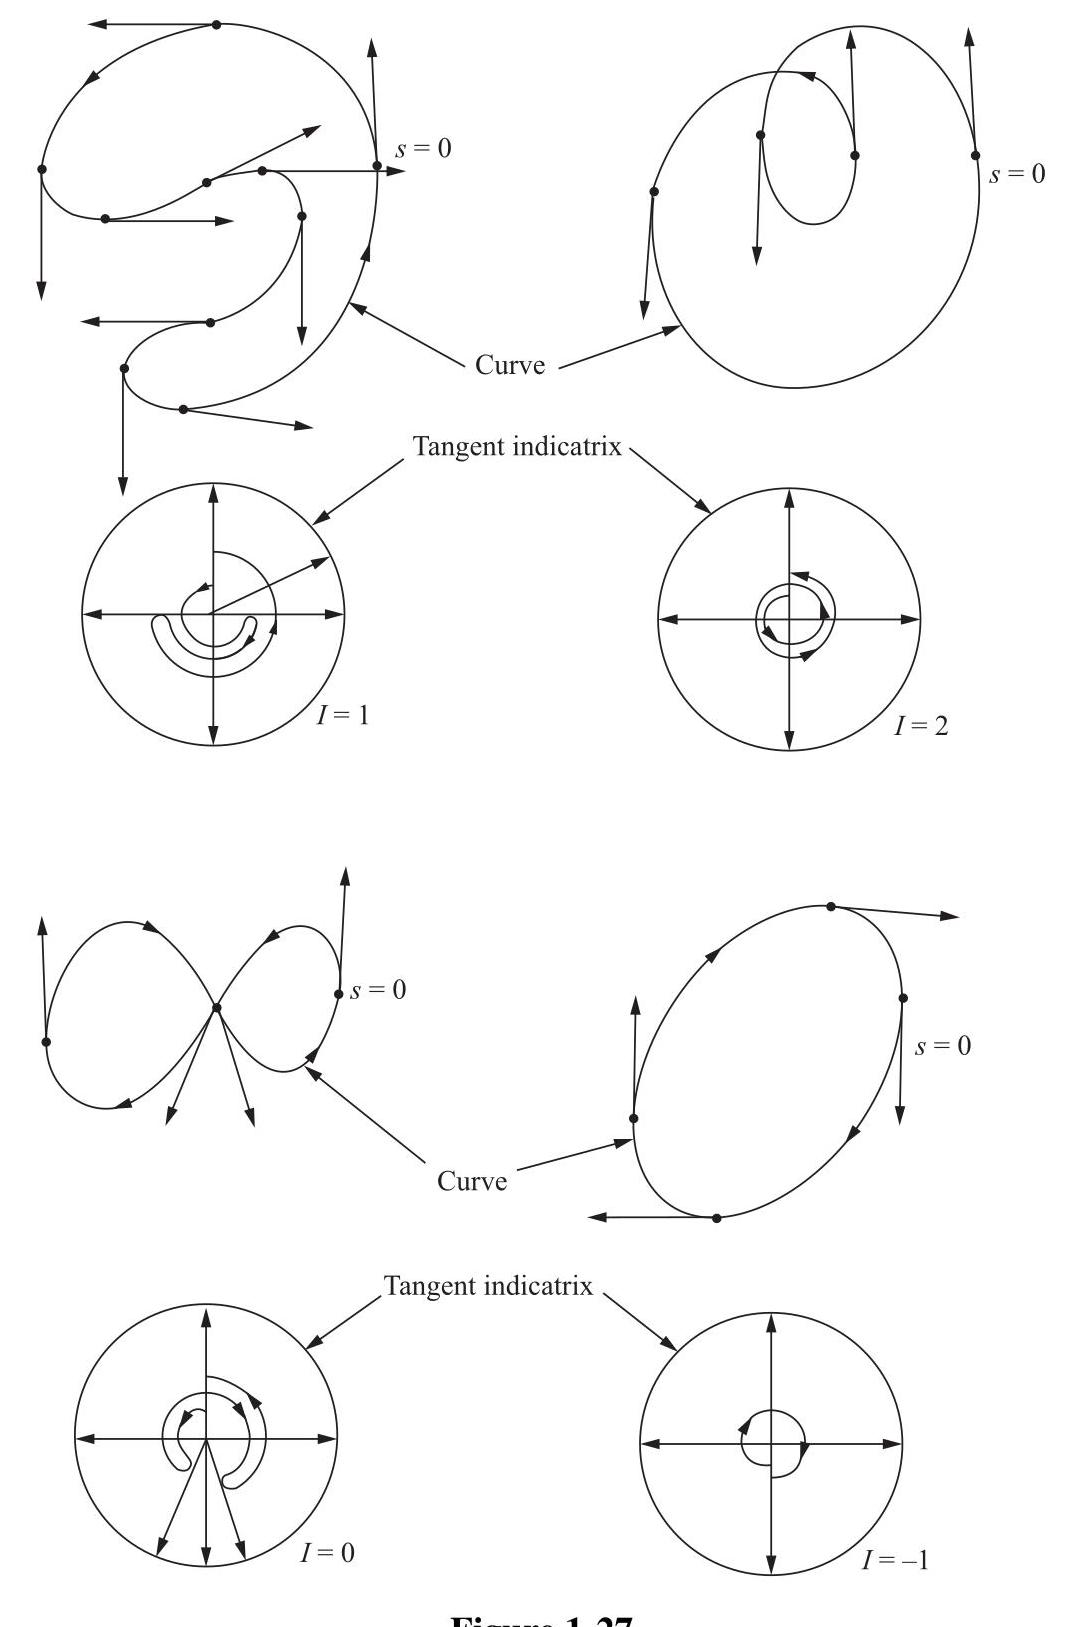
\includegraphics[max width=0.9\textwidth]{images/bo_d4b9jf3ef24c73e0334g_51_226_185_1080_1627_0.jpg}
\captionof{figure}{图 1-27}
\end{center}

\begin{center}
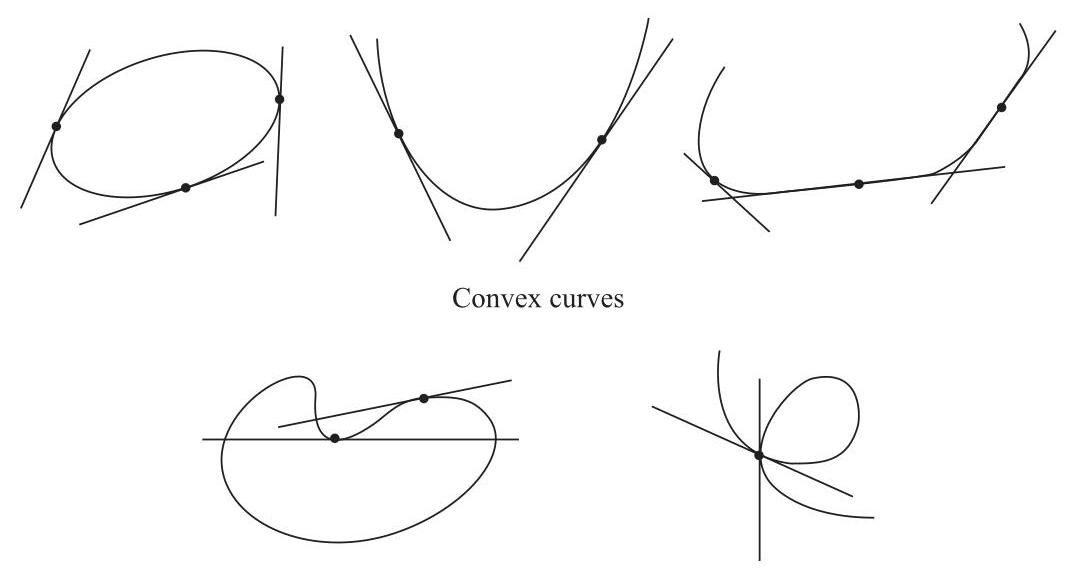
\includegraphics[max width=0.9\textwidth]{images/bo_d4b9jf3ef24c73e0334g_52_248_187_1073_568_0.jpg}
\captionof{figure}{非凸曲线}
\end{center}

定理证明.用弧长参数化曲线， \(\alpha  : \left\lbrack  {0,l}\right\rbrack   \rightarrow  {R}^{2}\) .由于 \(k = k\left( s\right)\) 是闭区间 \(\left\lbrack  {0,l}\right\rbrack\) 上的连续函数，它在该区间上会达到最大值和最小值(这是实函数中的一个基本事实；例如，可以在第 5 章附录，命题 13 中找到证明).因此， \(\alpha\) 至少有两个顶点， \(\alpha \left( {s}_{1}\right)  = p\) 和 \(\alpha \left( {s}_{2}\right)  = q\) .设 \(L\) 为通过 \(p\) 和 \(q\) 的直线，设 \(\beta\) 和 \(\gamma\) 为由点 \(p\) 和 \(q\) 确定的 \(\alpha\) 的两条弧.

我们声称这些弧中的每一个都位于 \(L\) 的一个确定侧.否则，它会在一个点 \(r\) 处与 \(L\) 相交，该点 \(r\) 不同于 \(p\) 和 \(q\) (图 1-29(a)).根据凸性，并且由于 \(p,q,r\) 是 \(C\) 上的不同点，中间点(例如 \(p\) )处的切线必须与 \(L\) 一致.同样，根据凸性，这意味着 \(L\) 在三个点 \(p,q\) 处与 \(C\) 相切，以及 \(r\) .但那样的话，靠近 \(p\) (中间点)的点的切线将使 \(q\) 和 \(r\) 位于不同的侧面，除非 \(L\) 的整个段 \({rq}\) 属于 \(C\) (图 1-29(b)).这意味着 \(p\) 和 \(q\) 处的 \(k = 0\) .由于这些是 \(C\) 上 \(k,k \equiv  0\) 的最大值和最小值点，因此出现矛盾.

设 \({Ax} + {By} + C = 0\) 为 \(L\) 的方程.如果没有进一步的顶点， \({k}^{\prime }\left( s\right)\) 在每个弧 \(\beta\) 和 \(\gamma\) 上保持恒定符号.然后我们可以调整所有系数 \(A,B,C\) 的符号，使得方程 (5) 中的积分是正的.这个矛盾表明存在第三个顶点，并且 \({k}^{\prime }\left( s\right)\) 在 \(\beta\) 或 \(\gamma\) 上改变符号，例如在 \(\beta\) 上.由于 \(p\) 和 \(q\) 是最大值和最小值点， \({k}^{\prime }\left( s\right)\) 在 \(\beta\) 上改变两次符号.因此，存在第四个顶点.Q.E.D.

四顶点定理一直是许多研究的主题.该定理也适用于简单、闭合(不一定是凸的)曲线，但证明更难.有关该主题的更多文献，请参阅参考文献 [10].

\begin{center}
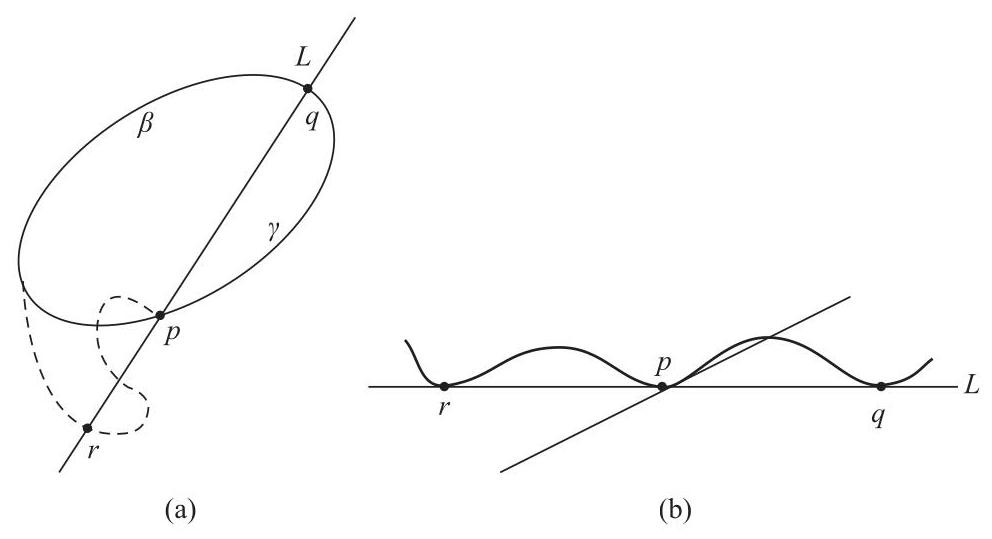
\includegraphics[max width=0.8\textwidth]{images/bo_d4b9jf3ef24c73e0334g_53_268_189_992_539_0.jpg}
\captionof{figure}{图 1-29}
\end{center}

稍后(第 5-7 节，命题 1)我们将证明平面闭合曲线是凸的当且仅当它是简单的并且可以定向使得其曲率为正或零.由此以及上述证明，我们看到可以将四顶点定理的陈述重新表述如下.闭合凸曲线的曲率函数是(非负的)并且要么是常数，要么至少有两个最大值和两个最小值.那么自然会问这样的曲率函数是否能表征凸曲线.更确切地说，我们可以问以下问题.设 \(\mathrm{k} : \left\lbrack  {\mathrm{a},\mathrm{b}}\right\rbrack   \rightarrow  \mathbb{R}\) 是一个可微的非负函数，使得 \(\mathrm{k}\) 在 \(\mathrm{a}\) 和 \(\mathrm{b}\) 处与其所有导数都一致.假设 \(\mathrm{k}\) 要么是常数，要么至少有两个最大值和两个最小值.是否存在一个简单的闭合曲线 \(\alpha  : \left\lbrack  {\mathrm{a},\mathrm{b}}\right\rbrack   \rightarrow  {\mathbb{R}}^{2}\) ，使得 \(\alpha\) 在 \(\mathrm{t}\) 处的曲率是 \(\mathrm{k}\left( \mathrm{t}\right)\) ？

对于 \(k\left( t\right)\) 严格为正的情况，H. Gluck 已肯定地回答了上述问题(参见 H. Gluck，“四顶点定理的逆定理”，L'Enseignement Mathématique T. XVII, fasc. 3-4 (1971), 295-309).然而，他的方法不适用于 \(k \geq  0\) 的情况.

\subsection*{C. 柯西-克罗夫顿公式}

本节的最后一个主题将致力于找到一个定理，该定理大致描述了以下情况.设 \(C\) 为平面中的一条正则曲线.我们考察所有与 \(C\) 相交的平面直线，并为每条这样的直线分配一个重数，该重数是它与 \(C\) 的交点数(图 1-30).

我们首先想找到一种方法来为平面上给定的直线子集分配一个度量.这并非令人惊讶，因为我们也可以为平面的点子集分配一个度量(面积).一旦我们意识到一条直线可以由两个参数确定(例如，图 1-31 中的 \(p\) 和 \(\theta\) )，我们就可以将平面上的直线视为某个平面区域中的点.因此，我们想要找到一种“合理”的方法来度量这样一个平面中的“面积”.

\begin{center}
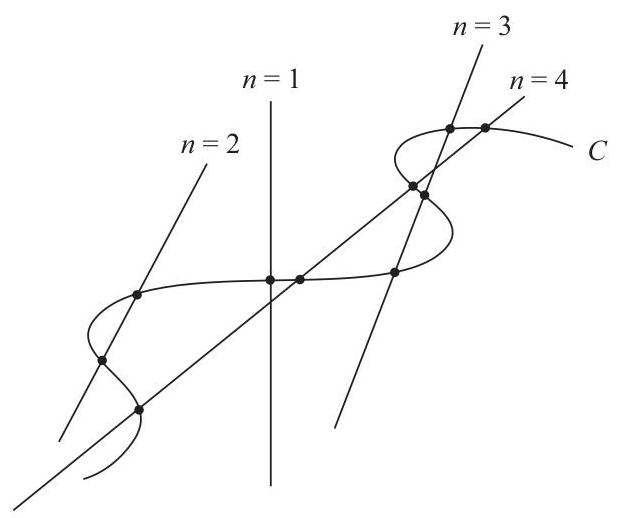
\includegraphics[max width=0.5\textwidth]{images/bo_d4b9jf3ef24c73e0334g_54_198_194_620_518_0.jpg}
\captionof{figure}{\(n\) 是相应直线的重数.}
\end{center}

\begin{center}
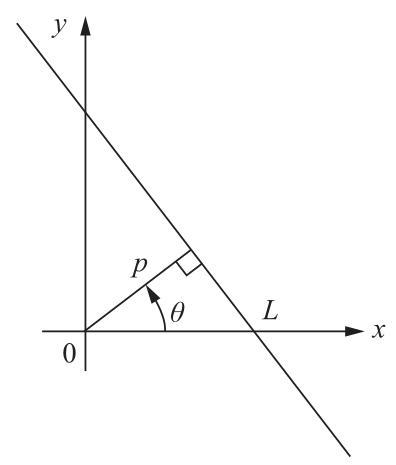
\includegraphics[max width=0.3\textwidth]{images/bo_d4b9jf3ef24c73e0334g_54_968_248_396_465_0.jpg}
\captionof{figure}{\(L\) 由 \(p\) 和 \(\theta\) 确定.}
\end{center}

选择了这种度量之后，我们想应用它并找到与 \(C\) 相交的直线集合(计入重数)的度量.结果相当有趣，可以表述如下.

定理 3(Cauchy-Crofton 公式).设 C 为一条正则平面曲线，其长度为 \(l\) .与 \(\mathrm{C}\) 相交的直线集合(计入重数)的度量等于 \({2l}\) .

在进入证明之前，我们必须定义在直线集合中什么是合理的度量.首先，让我们为这样的集合选择一个方便的坐标系.平面中的一条直线 \(L\) 由一条垂直于 \(L\) 的单位向量 \(v = \left( {\cos \theta ,\sin \theta }\right)\) 和 \(p = \; v \cdot  \alpha  = x\cos \theta  + y\sin \theta\) 与 \(L\) 的位置向量 \(v\) 的内积 \(\alpha  = \left( {x,y}\right)\) 来确定.请注意，为了用参数 \(\left( {p,\theta }\right)\) 来确定 \(L\) ，我们必须识别 \(\left( {p,\theta }\right)  \sim \; \left( {p,\theta  + {2k\pi }}\right) ,k\) (一个整数)，并且还必须识别 \(\left( {p,\theta }\right)  \sim  \left( {-p,\theta  \pm  \pi }\right)\) .

因此，我们可以用集合来代替平面上所有直线的集合

\[
\mathfrak{L} = \left\{  {\left( {p,\theta }\right)  \in  {R}^{2};\left( {p,\theta }\right)  \sim  \left( {p,\theta  + {2k\pi }}\right) \text{ and }\left( {p,\theta }\right)  \sim  \left( {-p,\theta  \pm  \pi }\right) }\right\}  .
\]

我们将证明，在选择单位的意义上，这个集合中只有一种合理的度量.

为了决定什么是合理的，让我们更仔细地看看 \({R}^{2}\) 中面积的通常度量.我们需要一个定义.

\({R}^{2}\) 中的刚性运动是一个映射 \(F : {R}^{2} \rightarrow  {R}^{2}\) ，由 \(\left( {\bar{x},\bar{y}}\right)  \rightarrow  \left( {x,y}\right)\) 给出，其中(图 1-32)

(6)
\[
x = a + \bar{x}\cos \varphi  - \bar{y}\sin \varphi
\]

\[
y = b + \bar{x}\sin \varphi  + \bar{y}\cos \varphi .
\]

\begin{center}
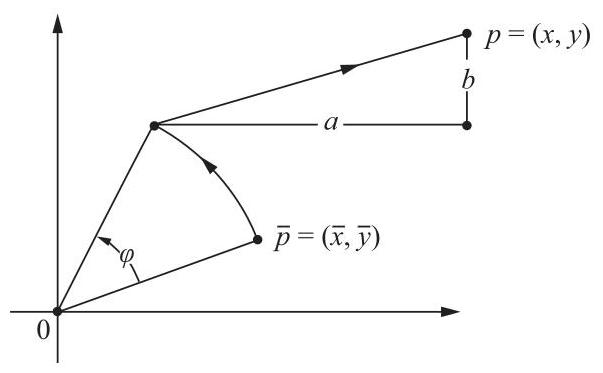
\includegraphics[max width=0.5\textwidth]{images/bo_d4b9jf3ef24c73e0334g_55_182_345_603_373_0.jpg}
\captionof{figure}{}
\end{center}

现在，为了定义集合 \(S \subset  {R}^{2}\) 的面积，我们考虑二重积分

\[
{\iint }_{S}{dxdy}
\]

也就是说，我们对 \(S\) 上的“面积元素” \({dxdy}\) 进行积分.当这个积分在某种意义上存在时，我们说 \(S\) 是可测的，并将 \(S\) 的面积定义为上述积分的值.从现在起，我们将假设我们讨论中涉及的所有积分都存在.

请注意，我们可以选择其他面积元素，例如 \(x{y}^{2}{dxdy}\) .选择 \({dxdy}\) 的原因是，在某个因子下，这是唯一在刚性运动下不变的面积元素.更准确地说，我们有以下命题.

命题 1.设 \(\mathrm{f}\left( {\mathrm{x},\mathrm{y}}\right)\) 是定义在 \({\mathbb{R}}^{2}\) 上的连续函数.对于任何集合 \(\mathrm{S} \subset  {\mathbb{R}}^{2}\) ，通过以下方式定义 \(\mathrm{S}\) 的面积 \(\mathrm{A}\) :

\[
A\left( S\right)  = {\iint }_{S}f\left( {x,y}\right) {dxdy}
\]

(当然，我们只考虑上述积分存在的集合).假设 \(\mathrm{A}\) 在刚体运动下不变；也就是说，如果 \(\mathrm{S}\) 是任意集合，而 \(\overline{\mathrm{S}} = {\mathrm{F}}^{-1}\left( \mathrm{\;S}\right)\) ，其中 \(\mathrm{F}\) 是刚体运动 (6)，那么

\[
\mathrm{A}\left( \overline{\mathrm{S}}\right)  = {\iint }_{\overline{\mathrm{S}}}\mathrm{f}\left( {\overline{\mathrm{x}},\overline{\mathrm{y}}}\right) \mathrm{d}\overline{\mathrm{x}}\mathrm{d}\overline{\mathrm{y}} = {\iint }_{\mathrm{S}}\mathrm{f}\left( {\mathrm{x},\mathrm{y}}\right) \mathrm{{dx}}\mathrm{{dy}} = \mathrm{A}\left( \mathrm{S}\right) .
\]

则 \(\mathrm{f}\left( {\mathrm{x},\mathrm{y}}\right)  =\) 为常数.

证明.我们回顾多重积分变量替换公式(Buck，《高等微积分》，第 301 页，或本节练习 15):

\[
{\iint }_{S}f\left( {x,y}\right) {dxdy} = {\iint }_{\bar{S}}f\left( {x\left( {\bar{x},\bar{y}}\right) ,y\left( {\bar{x},\bar{y}}\right) }\right) \frac{\partial \left( {x,y}\right) }{\partial \left( {\bar{x},\bar{y}}\right) }d\bar{x}d\bar{y}. \tag{7}
\]

其中， \(x = x\left( {\bar{x},\bar{y}}\right) ,y = y\left( {\bar{x},\bar{y}}\right)\) 是具有连续偏导数的函数，它们定义了变量 \(T : {R}^{2} \rightarrow  {R}^{2},\bar{S} = {T}^{-1}\left( S\right)\) 的变换，并且

\[
\frac{\partial \left( {x,y}\right) }{\partial \left( {\bar{x},\bar{y}}\right) } = \left| \begin{array}{ll} \frac{\partial x}{\partial \bar{x}} & \frac{\partial x}{\partial \bar{y}} \\  \frac{\partial y}{\partial \bar{x}} & \frac{\partial y}{\partial \bar{y}} \end{array}\right|
\]

是变换 \(T\) 的雅可比行列式.在我们的特定情况下，变换是刚体运动(6)，雅可比行列式为

\[
\frac{\partial \left( {x,y}\right) }{\partial \left( {\bar{x},\bar{y}}\right) } = \left| \begin{array}{rr} \cos \varphi &  - \sin \varphi \\  \sin \varphi & \cos \varphi  \end{array}\right|  = 1.
\]

利用这一事实和公式(7)，我们得到

\[
{\iint }_{\bar{S}}f\left( {x\left( {\bar{x},\bar{y}}\right) ,y\left( {\bar{x},\bar{y}}\right) }\right) d\bar{x}d\bar{y} = {\iint }_{\bar{S}}f\left( {\bar{x},\bar{y}}\right) d\bar{x}d\bar{y}.
\]

由于这对所有 \(S\) 都成立，我们有

\[
f\left( {x\left( {\bar{x},\bar{y}}\right) ,y\left( {\bar{x},\bar{y}}\right) }\right)  = f\left( {\bar{x},\bar{y}}\right) .
\]

我们现在利用这样一个事实:对于 \({R}^{2}\) 中的任意两点 \(\left( {x,y}\right) ,\left( {\bar{x},\bar{y}}\right)\) ，都存在一个刚体运动 \(F\) ，使得 \(F\left( {\bar{x},\bar{y}}\right)  = \left( {x,y}\right)\) .因此，

\[
f\left( {x,y}\right)  = \left( {f \circ  F}\right) \left( {\bar{x},\bar{y}}\right)  = f\left( {\bar{x},\bar{y}}\right) ,
\]

且 \(f\left( {x,y}\right)  =\) 为常数，正如我们所期望的.Q.E.D.

注 3.上述证明基于两个事实:第一，刚体运动的雅可比行列式为 1；第二，刚体运动在平面点上传递；也就是说，给定平面上的任意两点，都存在一个刚体运动将一点映射到另一点.

有了这些准备，我们终于可以在集合 \(\mathfrak{L}\) 中定义一个测度了.我们首先观察到刚体运动(6)在 \(\mathfrak{L}\) 上诱导了一个变换.事实上，公式(6)将直线 \(x\cos \theta  + y\sin \theta  = p\) 映射到直线

\[
\bar{x}\cos \left( {\theta  - \varphi }\right)  + \bar{y}\sin \left( {\theta  - \varphi }\right)  = p - a\cos \theta  - b\sin \theta .
\]

这意味着 Eq. (6) 诱导的变换作用于 \(\mathfrak{L}\) 的结果是

\[
\bar{p} = p - a\cos \theta  - b\sin \theta ,
\]

\[
\overline{\theta } = \theta  - \varphi
\]

可以轻松验证上述变换的雅可比行列式为 1，并且此类变换在平面上的直线集合上也是可传递的.然后我们定义集合 \(\mathfrak{S} \subset  \mathfrak{L}\) 的测度为

\[
{\iint }_{\mathfrak{S}}{dpd\theta }
\]

与命题 1 的情况相同，我们可以证明，在常数因子下，这是 \(\mathfrak{L}\) 上在刚体运动下不变的唯一测度.因此，这个测度尽可能合理.

现在我们可以勾勒出定理 3 的证明.

定理 3 证明草图.首先假设曲线 \(C\) 是长度为 \(l\) 的直线段.由于我们的测度在刚体运动下不变，我们可以假设坐标系的原点 0 位于 \(C\) 的中点，并且 \(x\) 轴沿 \(C\) 的方向.那么与 \(C\) 相交的直线集合的测度为(图 1-33)

\[
\iint {dpd\theta } = {\int }_{0}^{2\pi }\left( {{\int }_{0}^{\left| {\cos \theta }\right| \left( {l/2}\right) }{dp}}\right) {d\theta } = {\int }_{0}^{2\pi }\frac{l}{2}\left| {\cos \theta }\right| {d\theta } = {2l}.
\]

\begin{center}
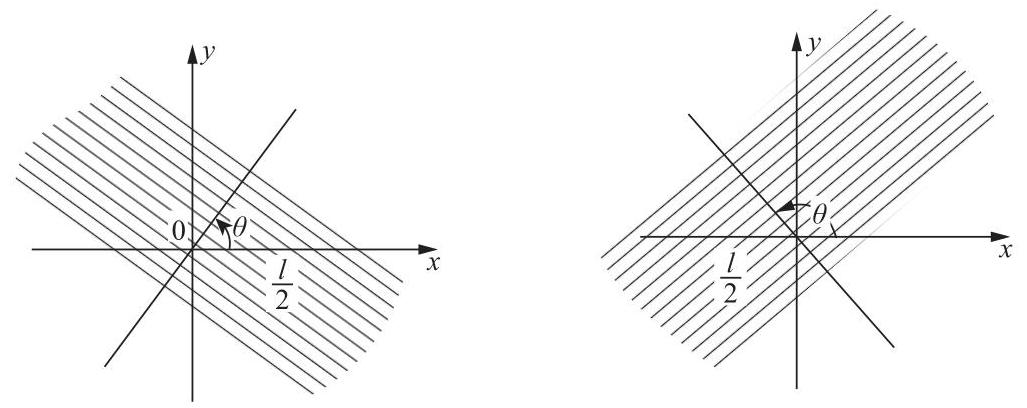
\includegraphics[max width=0.9\textwidth]{images/bo_d4b9jf3ef24c73e0334g_57_254_1462_1027_408_0.jpg}
\captionof{figure}{}
\end{center}

接下来，设 \(C\) 是由有限数量的长度为 \({l}_{i}\left( {\sum {l}_{i} = l}\right)\) 的线段 \({C}_{i}\) 组成的折线.设 \(n = n\left( {p,\theta }\right)\) 是直线 \(\left( {p,\theta }\right)\) 与 \(C\) 的交点数.然后，通过对每条线段 \({C}_{i}\) 的结果求和，我们得到

\[
\iint {ndpd\theta } = 2\mathop{\sum }\limits_{i}{l}_{i} = {2l}, \tag{8}
\]

这就是折线的柯西-克罗夫顿公式.

最后，通过极限过程，可以将上述公式推广到任何正则曲线，这将证明定理 3.Q.E.D.

应该指出的是，这个主题的一般思想属于几何学的一个分支，称为积分几何.该主题的概述可以在 L. A. Santaló 的《积分几何》中找到，收录于 S. S. Chern 编辑的《全球几何与分析研究》一书中，数学协会，1967 年，页码 147-193.

柯西-克罗夫顿公式可以以多种方式使用.例如，如果一条曲线不可求长(参见练习 9，第 1-3 节)，但等式 (8) 的左侧有意义，则可用于定义此类曲线的“长度”.等式 (8) 也可用于获得估计曲线长度的有效方法.事实上，等式 (8) 中积分的一个良好近似如下. \({}^{ \dagger  }\) 考虑一组平行直线，使得两条连续直线之间的距离为 \(r\) .将这组直线旋转 \(\pi /4,{2\pi }/4,{3\pi }/4\) 的角度，以获得四组直线.设 \(n\) 是曲线 \(C\) 与所有这些直线的交点数.那么

\[
\frac{1}{2}{nr}\frac{\pi }{4}
\]

是积分的近似值

\[
\frac{1}{2}\iint {ndpd\theta } = \text{ length of }C
\]

因此给出了 \(C\) 长度的估计值.为了了解这个估计值有多好，让我们举个例子.

示例.图 1-34 是一个圆形 DNA 分子的电子显微照片，我们想估计其长度.在图片上绘制了距离为 7 毫米且角度为 \(\pi /4\) 的四组直线(更实用的方法是将这组直线一次性绘制在透明纸上).发现交点数为 153.因此，

\[
\frac{1}{2}n\frac{\pi }{4} = \frac{1}{2}{153}\frac{3.14}{4} \sim  {60}
\]



†我感谢 Robert Gardner (1939-1998) 提出此应用及后续示例.



\begin{center}
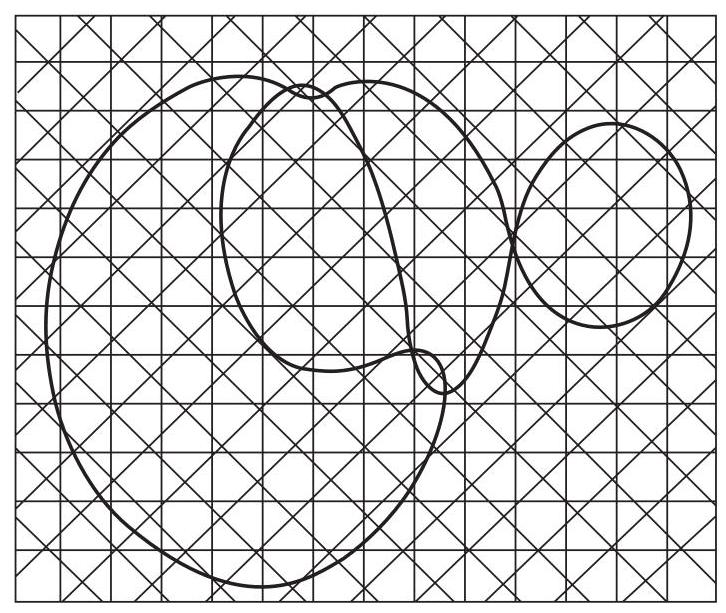
\includegraphics[max width=0.6\textwidth]{images/bo_d4b9jf3ef24c73e0334g_59_401_189_726_613_0.jpg}
\captionof{figure}{转载自 H. Ris 和 B. C. Chandler 的 Cold Spring Harbor Symp. Quant. Biol. 28, 2 (1963)，经许可.}
\end{center}

由于图中参考线代表1微米 \(\left( { = {10}^{-6}}\right.\) 米 \()\) ，并且按我们的比例尺测量为25毫米， \(r = \frac{7}{25}\) ，因此，根据我们的数值，该DNA分子的长度近似为

\[
{60}\left( \frac{7}{25}\right)  = {16.8}\text{ micrometers. }
\]

实际值为16.3微米.

\exerciseline

*1. 平面内是否存在一条长度为6英尺且围成3平方英尺面积的简单闭合曲线？

*2. 设 \(\overline{AB}\) 为一条直线段，设 \(l >\) 为 \({AB}\) 的长度.证明连接 \(A\) 和 \(B\) 的曲线 \(C\) ，其长度为 \(l\) ，并且与 \(\overline{AB}\) 一起围成最大可能面积，是一条通过 \(A\) 和 \(B\) 的圆弧(图1-35).

\begin{center}
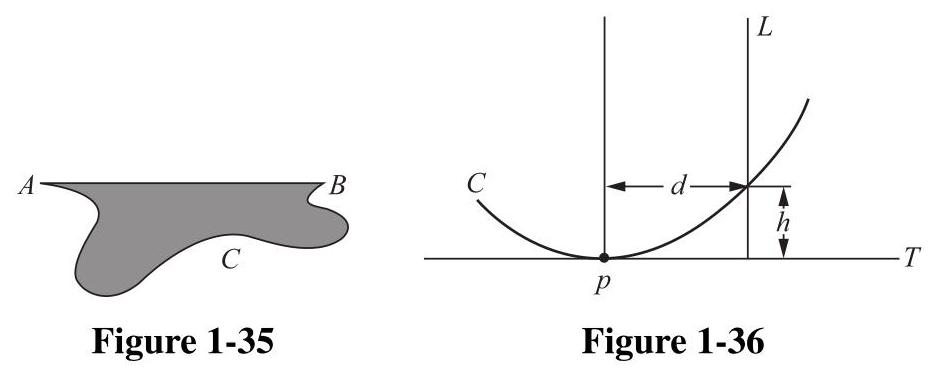
\includegraphics[max width=0.8\textwidth]{images/bo_d4b9jf3ef24c73e0334g_60_307_195_933_373_0.jpg}
\captionof{figure}{}
\end{center}
\hspace*{3em} 

3. 计算椭圆的曲率

\[
x = a\cos t,\;y = b\sin t,\;t \in  \left\lbrack  {0,{2\pi }}\right\rbrack  ,a \neq  b,
\]

并证明它恰好有四个顶点，即点 \(\left( {a,0}\right)\) ， \(\left( {-a,0}\right) ,\left( {0,b}\right) ,\left( {0, - b}\right)\) .

*4. 设 \(C\) 为一条平面曲线，设 \(T\) 为某点 \(p \in  C\) 处的切线.画一条与 \(p\) 处的法线 \(L\) 平行且距离 \(p\) 为 \(d\) 的直线(图1-36).设 \(h\) 是 \(C\) 和 \(T\) 在 \(L\) 上确定的线段的长度(因此， \(h\) 是 \(C\) 相对于 \(T\) 的“高度”).证明

\[
\left| {k\left( p\right) }\right|  = \mathop{\lim }\limits_{{d \rightarrow  0}}\frac{2h}{{d}^{2}}
\]

其中 \(k\left( p\right)\) 是 \(C\) 在 \(p\) 处的曲率.

*5. 如果一条闭合平面曲线 \(C\) 包含在一个半径为 \(r\) 的圆盘内，证明存在一点 \(p \in  C\) ，使得 \(C\) 在 \(p\) 处的曲率 \(k\) 满足 \(\left| k\right|  \geq  1/r\) .

6. 设 \(\alpha \left( s\right) ,s \in  \left\lbrack  {0,l}\right\rbrack\) 为一条正向的闭合凸平面曲线.曲线

\[
\beta \left( s\right)  = \alpha \left( s\right)  - {rn}\left( s\right) ,
\]

其中 \(r\) 为正常数， \(n\) 为法向量，称为 \(\alpha\) 的平行曲线(图1-37).证明

a. \(\beta  =\) 的长度等于 \(\alpha  + {2\pi r}\) 的长度.

b. \(A\left( \beta \right)  = A\left( \alpha \right)  + {rl} + \pi {r}^{2}\) .

c. \({k}_{\beta }\left( s\right)  = {k}_{\alpha }\left( s\right) /\left( {1 + r{k}_{\alpha }\left( s\right) }\right)\) .

对于(a)-(c)， \(A\) (   )表示相应曲线所围成的面积，而 \({k}_{\alpha },{k}_{\beta }\) 和 \(\beta\) 分别是 \(\alpha\) 和 \(\beta\) 的曲率.

7. 设 \(\alpha  : R \rightarrow  {R}^{2}\) 为在整个实数轴 \(R\) 上定义的平面曲线.假设 \(\alpha\) 不经过原点 \(0 = \left( {0,0}\right)\) ，并且两者都

\[
\mathop{\lim }\limits_{{t \rightarrow   + \infty }}\left| {\alpha \left( t\right) }\right|  = \infty \;\text{ and }\;\mathop{\lim }\limits_{{t \rightarrow   - \infty }}\left| {\alpha \left( t\right) }\right|  = \infty .
\]

\begin{center}
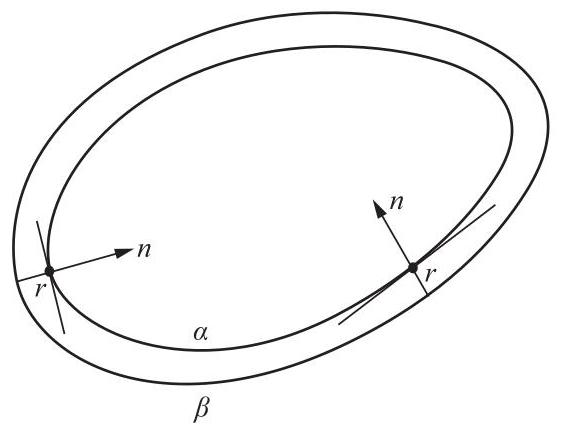
\includegraphics[max width=0.5\textwidth]{images/bo_d4b9jf3ef24c73e0334g_61_180_193_561_438_0.jpg}
\captionof{figure}{图1-37}
\end{center}

a. 证明存在一点 \({t}_{0} \in  R\) 使得对于所有 \(t \in  R\) 都有 \(\left| {\alpha \left( {t}_{0}\right) }\right|  \leq  \left| {\alpha \left( t\right) }\right|\) .

b. 用一个例子说明，如果不假设 \(\mathop{\lim }\limits_{{t \rightarrow   + \infty }}\left| {\alpha \left( t\right) }\right|  = \infty\) 和 \(\mathop{\lim }\limits_{{t \rightarrow   - \infty }}\left| {\alpha \left( t\right) }\right|  = \infty\) ，则 a 部分的论断是错误的.

8.*a. 令 \(\alpha \left( s\right) ,s \in  \left\lbrack  {0,l}\right\rbrack\) 为一个平面简单闭合曲线.假设曲率 \(k\left( s\right)\) 满足 \(0 < k\left( s\right)  \leq  c\) ，其中 \(c\) 是一个常数(因此， \(\alpha\) 的曲率小于半径为 \(1/c\) 的圆).证明:

\[
\text{ length of }\alpha  \geq  \frac{2\pi }{c}\text{ . }
\]

b. 在 a 部分中，将简单闭合的假设替换为“ \(\alpha\) 的旋转指数为 \(N\) ”.证明:

\[
\text{ length of }\alpha  \geq  \frac{2\pi N}{c}\text{ . }
\]

*9. 如果给定任意两点 \(p,q \in  K\) ，直线 \(\overline{pq}\) 的线段包含在 \(K\) 中，则称集合 \(K \subset  {R}^{2}\) 是凸集(图 1-38).证明一个简单的闭合凸曲线围成一个凸集.

10. 令 \(C\) 为一个凸平面曲线.几何证明 \(C\) 没有自交点.

*11. 给定一条非凸的简单闭合平面曲线 \(C\) ，我们可以考虑它的凸包 \(H\) (图 1-39)，即包含 \(C\) 内部的最小凸集的边界.曲线 \(H\) 由 \(C\) 的弧段和连接“非凸间隙”的切线段组成(图 1-39).可以证明 \(H\) 是一条 \({C}^{1}\) 闭合凸曲线.利用这一点说明，在等周问题中，我们可以限制于凸曲线.

*12. 考虑平面上的单位圆 \({S}^{1}\) .证明比率 \({M}_{1}/{M}_{2} = \frac{1}{2}\) ，其中 \({M}_{2}\) 是平面上与 \({S}^{1}\) 相交的直线集合的测度，而 \({M}_{1}\) 是所有在 \({S}^{1}\) 中确定长度为 \(> \sqrt{3}\) 的弦的此类直线的测度.直观地说，这个比率是与 \({S}^{1}\) 相交的直线在 \({S}^{1}\) 中确定比内接于 \({S}^{1}\) 的等边三角形边长更长的弦的概率(图 1-40).

\begin{center}
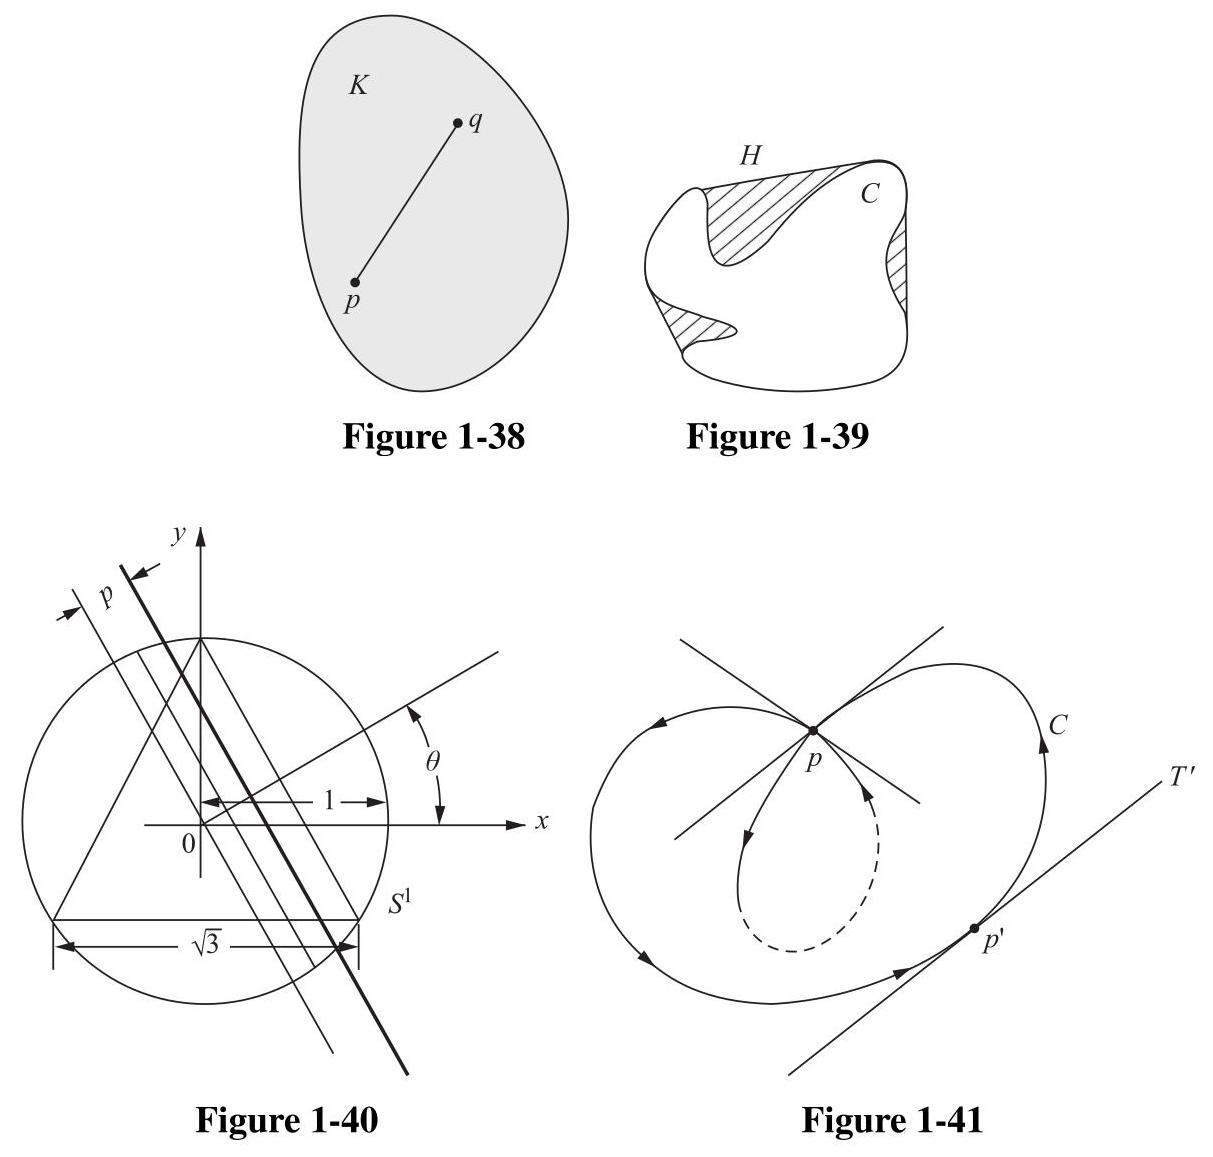
\includegraphics[max width=1.0\textwidth]{images/bo_d4b9jf3ef24c73e0334g_62_191_190_1213_1157_0.jpg}
\end{center}
\hspace*{3em} 

13. 令 \(C\) 为一个有向平面闭合曲线，其曲率为 \(k > 0\) .假设 \(C\) 至少有一个自交点 \(p\) .证明:

a. 存在一点 \({p}^{\prime } \in  C\) ，使得在 \({p}^{\prime }\) 处的切线 \({T}^{\prime }\) 平行于某处 \(p\) 的切线.

b. 在 \(p{p}^{\prime }p\) 构成的 \(C\) 的正向弧段中，切线的旋转角度为 \(> \pi\) (图 1-41).

c. \(C\) 的旋转指数为 \(\geq  2\) .

14. a. 说明如果一条直线 \(L\) 与一个闭合凸曲线 \(C\) 相交，那么 \(L\) 要么是 \(C\) 的切线，要么 \(L\) 与 \(C\) 精确地相交于两点.

b. 利用 a 部分说明与 \(C\) 相交的直线集合的测度(不计重数)等于 \(C\) 的长度.

平面上的格林公式是微积分中的一个基本事实，可以表述如下.设一条简单的闭合平面曲线由 \(\alpha \left( t\right)  = \; \left( {x\left( t\right) ,y\left( t\right) }\right) ,t \in  \left\lbrack  {a,b}\right\rbrack\) 给出.假设 \(\alpha\) 是正向定向的，设 \(C\) 是它的轨迹，设 \(R\) 是 \(C\) 的内部.设 \(p = p\left( {x,y}\right) ,q = q\left( {x,y}\right)\) 是具有连续偏导数 \({p}_{x},{p}_{y},{q}_{x},{q}_{y}\) 的实函数.则

\[
{\iint }_{R}\left( {{q}_{x} - {p}_{y}}\right) {dxdy} = {\int }_{C}\left( {p\frac{dx}{dt} + q\frac{dy}{dt}}\right) {dt}, \tag{9}
\]

其中第二个积分理解为函数 \(p\) 和 \(q\) 被限制在 \(\alpha\) 上，积分在极限 \(t = a\) 和 \(t = b\) 之间取值.在下面的 a 和 b 部分，我们建议从格林公式推导出 \(R\) 的面积公式以及重积分变量替换公式(参见文中的公式 (1) 和 (7)).

a. 在公式 (9) 中设置 \(q = x\) 和 \(p =  - y\) ，并得出

\[
A\left( R\right)  = {\iint }_{R}{dxdy} = \frac{1}{2}{\int }_{a}^{b}\left( {x\left( t\right) \frac{dy}{dt} - y\left( t\right) \frac{dx}{dt}}\right) {dt}.
\]

b. 设 \(f\left( {x,y}\right)\) 是一个具有连续偏导数的实函数，而 \(T : {R}^{2} \rightarrow  {R}^{2}\) 是由函数 \(x = x\left( {u,v}\right) ,y = y\left( {u,v}\right)\) 给出的坐标变换，这些函数也具有连续偏导数.在公式 (9) 中选择 \(p = 0\) 和 \(q\) ，使得 \({q}_{x} = f\) .依次应用格林公式、映射 \(T\) 和格林公式再次得到

\[
{\iint }_{R}f\left( {x,y}\right) {dxdy}
\]

\[
= {\int }_{C}{qdy} = {\int }_{{T}^{-1}\left( C\right) }\left( {q \circ  T}\right) \left( {{y}_{u}{u}^{\prime }\left( t\right)  + {y}_{v}{v}^{\prime }\left( t\right) }\right) {dt}
\]

\[
= {\iint }_{{T}^{-1}\left( R\right) }\left\{  {\frac{\partial }{\partial u}\left( {\left( {q \circ  T}\right) {y}_{v}}\right)  - \frac{\partial }{\partial v}\left( {\left( {q \circ  T}\right) {y}_{u}}\right) }\right\}  {dudv}.
\]

证明

\[
\frac{\partial }{\partial u}\left( {q\left( {x\left( {u,v}\right) ,y\left( {u,v}\right) }\right) {y}_{v}}\right)  - \frac{\partial }{\partial v}\left( {q\left( {x\left( {u,v}\right) ,y\left( {u,v}\right) }\right) {y}_{u}}\right)
\]

\[
= f\left( {x\left( {u,v}\right) ,y\left( {u,v}\right) }\right) \left( {{x}_{u}{y}_{v} - {x}_{v}{y}_{u}}\right)  = f\frac{\partial \left( {x,y}\right) }{\partial \left( {u,v}\right) }.
\]

将此与上述结果结合起来，得到重积分的变换公式:

\[
{\iint }_{R}f\left( {x,y}\right) {dxdy} = {\iint }_{{T}^{-1}\left( R\right) }f\left( {x\left( {u,v}\right) ,y\left( {u,v}\right) }\right) \frac{\partial \left( {x,y}\right) }{\partial \left( {u,v}\right) }{dudv}.
\]